\synctex=1
\documentclass[11pt,aspectratio=169]{beamer}

\usepackage[T1]{fontenc}
\usepackage[french,provide=*]{babel}
\usepackage{amsmath,amssymb,amsfonts}
\usepackage{mathtools}
\usepackage{bm}
\usepackage{pgfplots}
\usepackage{xcolor}
\pgfplotsset{compat=1.18}

% Police serif pour les mathématiques
\usefonttheme[onlymath]{serif}

% Couleurs
\definecolor{gray}{gray}{0.4}

% Différentielle droite
\newcommand{\dd}{\mathrm{d}}

% Git hash
\usepackage{xstring}
\usepackage{catchfile}
\immediate\write18{git rev-parse HEAD > git.hash}
\CatchFileDef{\HEAD}{git.hash}{\endlinechar=-1}
\newcommand{\gitrevision}{\StrLeft{\HEAD}{7}}

\usepackage{ccicons}

% Pied de page personnalisé
\setbeamertemplate{footline}{
  \hfill\vspace*{1pt}\href{https://creativecommons.org/publicdomain/zero/1.0/deed.fr}{\cczero}\enspace\href{https://github.com/stepan-a/microeconometrics}{\gitrevision}\enspace--\enspace\insertframenumber/\inserttotalframenumber\enspace--\enspace\today\enspace}

% Supprimer la barre de navigation
\setbeamertemplate{navigation symbols}{}

\title{Estimation par Maximum de Vraisemblance}
\subtitle{Exemples}
\author{}
\date{}
\institute{}

\AtBeginSection[]
{
  \begin{frame}
    \frametitle{Plan}
    \tableofcontents[currentsection]
  \end{frame}
}

\begin{document}

\begin{frame}
\titlepage
\end{frame}

\begin{frame}{Plan}
\tableofcontents
\end{frame}

%==============================================================================
\section{Loi normale}
%==============================================================================

\begin{frame}{Loi normale -- Présentation}

\begin{itemize}

\item La loi normale est omniprésente en statistique :\newline
  \begin{itemize}
    \item Erreurs de mesure en physique, métrologie\newline
    \item Taille, poids et caractéristiques biologiques\newline
    \item Scores de tests psychométriques\newline
    \item Rendements financiers (en première approximation)\newline
    \item Distribution limite par le théorème central limite\newline
  \end{itemize}

\item C'est la distribution de référence pour la théorie de l'estimation : c'est souvent le cas où les calculs sont les plus explicites.

\end{itemize}

\end{frame}

\begin{frame}{Loi normale -- Modèle}

\begin{itemize}

\item $X_i \sim \mathcal{N}(\mu, \sigma^2)$ avec $\mu \in \mathbb{R}$ et $\sigma^2 > 0$ :
  \[
  f(x; \mu, \sigma^2) = \frac{1}{\sigma\sqrt{2\pi}} \exp\left(-\frac{(x-\mu)^2}{2\sigma^2}\right)
  \]

\item Moments :
  \[
  \mathbb{E}[X] = \mu, \qquad \mathbb{V}[X] = \sigma^2
  \]

\item On peut paramétrer par $(\mu, \sigma^2)$ ou par $(\mu, \sigma)$. Nous utilisons $(\mu, \sigma^2)$.

\end{itemize}

\end{frame}

\begin{frame}{Loi normale -- Log-vraisemblance}

\begin{itemize}

\item Vraisemblance :
  \[
  L(\mu, \sigma^2) = \prod_{i=1}^n \frac{1}{\sigma\sqrt{2\pi}} \exp\left(-\frac{(x_i-\mu)^2}{2\sigma^2}\right)
  \]

\item Log-vraisemblance :
  \[
  \ell(\mu, \sigma^2) = -\frac{n}{2}\log(2\pi) - \frac{n}{2}\log(\sigma^2) - \frac{1}{2\sigma^2}\sum_{i=1}^n (x_i - \mu)^2
  \]

\item On peut réécrire le dernier terme :
  \[
  \sum_{i=1}^n (x_i - \mu)^2 = \sum_{i=1}^n (x_i - \bar{x})^2 + n(\bar{x} - \mu)^2
  \]

\end{itemize}

\end{frame}

\begin{frame}{Loi normale -- Estimateur de $\mu$}

\begin{itemize}

\item Condition du premier ordre :
  \[
  \frac{\partial \ell}{\partial \mu} = \frac{1}{\sigma^2}\sum_{i=1}^n (x_i - \mu) = 0 \quad \Rightarrow \quad \sum_{i=1}^n x_i = n\mu
  \]

\item Solution :
  \[
  \boxed{\hat{\mu}_{MV} = \frac{1}{n}\sum_{i=1}^n X_i = \bar{X}}
  \]

\item C'est la moyenne empirique.

\end{itemize}

\end{frame}

\begin{frame}{Loi normale -- Estimateur de $\sigma^2$}

\begin{itemize}

\item Condition du premier ordre :
  \[
  \frac{\partial \ell}{\partial \sigma^2} = -\frac{n}{2\sigma^2} + \frac{1}{2\sigma^4}\sum_{i=1}^n (x_i - \mu)^2 = 0
  \]

\item En remplaçant $\mu$ par $\hat{\mu} = \bar{x}$ :
  \[
  \frac{n}{2\sigma^2} = \frac{1}{2\sigma^4}\sum_{i=1}^n (x_i - \bar{x})^2
  \]

\item Solution :
  \[
  \boxed{\hat{\sigma}^2_{MV} = \frac{1}{n}\sum_{i=1}^n (X_i - \bar{X})^2}
  \]

\item C'est la variance empirique (avec diviseur $n$, pas $n-1$).

\end{itemize}

\end{frame}

\begin{frame}{Loi normale -- Distribution exacte de $\hat{\mu}$}

\begin{itemize}

\item Puisque $\hat{\mu} = \frac{1}{n}\sum_{i=1}^n X_i$ est une combinaison linéaire de variables normales indépendantes :
  \[
  \hat{\mu} \sim \mathcal{N}\left(\mu, \frac{\sigma^2}{n}\right)
  \]

\item Propriétés :
  \begin{itemize}
    \item $\mathbb{E}[\hat{\mu}] = \mu$ : estimateur sans biais\newline
    \item $\mathbb{V}[\hat{\mu}] = \dfrac{\sigma^2}{n}$ : variance exacte\newline
    \item Distribution exactement normale pour tout $n$
  \end{itemize}

\end{itemize}

\end{frame}

\begin{frame}{Loi normale -- Distribution exacte de $\hat{\sigma}^2$}

\begin{itemize}

\item On montre que :
  \[
  \frac{n\hat{\sigma}^2}{\sigma^2} = \frac{\sum_{i=1}^n (X_i - \bar{X})^2}{\sigma^2} \sim \chi^2_{n-1}
  \]

\item Puisque $\mathbb{E}[\chi^2_{n-1}] = n-1$ :
  \[
  \mathbb{E}\left[\frac{n\hat{\sigma}^2}{\sigma^2}\right] = n-1 \quad \Rightarrow \quad \mathbb{E}[\hat{\sigma}^2] = \frac{n-1}{n}\sigma^2
  \]

\item L'estimateur MV est biaisé : il sous-estime $\sigma^2$.\newline

\item Biais : $\text{Biais}(\hat{\sigma}^2) = -\dfrac{\sigma^2}{n}$

\end{itemize}

\end{frame}

\begin{frame}{Loi normale -- Estimateur sans biais de $\sigma^2$}

\begin{itemize}

\item L'estimateur sans biais de $\sigma^2$ est :
  \[
  \boxed{S^2 = \frac{1}{n-1}\sum_{i=1}^n (X_i - \bar{X})^2 = \frac{n}{n-1}\hat{\sigma}^2_{MV}}
  \]

\item On a $\mathbb{E}[S^2] = \sigma^2$.\newline

\item Le diviseur $n-1$ (et non $n$) correspond aux degrés de liberté : on perd un degré de liberté en estimant $\mu$ par $\bar{X}$.\newline

\item C'est l'estimateur utilisé par défaut dans la plupart des logiciels statistiques.

\end{itemize}

\end{frame}

\begin{frame}{Loi normale -- Variance de $\hat{\sigma}^2$}

\begin{itemize}

\item Puisque $\mathbb{V}[\chi^2_k] = 2k$, on a $\mathbb{V}[\chi^2_{n-1}] = 2(n-1)$.\newline

\item Variance de l'estimateur MV :
  \[
  \mathbb{V}\left[\frac{n\hat{\sigma}^2}{\sigma^2}\right] = 2(n-1) \quad \Rightarrow \quad \frac{n^2}{\sigma^4}\mathbb{V}[\hat{\sigma}^2] = 2(n-1)
  \]
  \[
  \boxed{\mathbb{V}[\hat{\sigma}^2] = \frac{2(n-1)\sigma^4}{n^2}}
  \]

\item Pour $n$ grand : $\mathbb{V}[\hat{\sigma}^2] \approx \dfrac{2\sigma^4}{n}$

\end{itemize}

\end{frame}

\begin{frame}{Loi normale -- Variance de $S^2$}

\begin{itemize}

\item Puisque $S^2 = \frac{n}{n-1}\hat{\sigma}^2$ :
  \[
  \mathbb{V}[S^2] = \frac{n^2}{(n-1)^2}\mathbb{V}[\hat{\sigma}^2] = \frac{n^2}{(n-1)^2} \cdot \frac{2(n-1)\sigma^4}{n^2}
  \]
  \[
  \boxed{\mathbb{V}[S^2] = \frac{2\sigma^4}{n-1}}
  \]

\item Pour $n$ grand, $\mathbb{V}[\hat{\sigma}^2_{MV}] < \mathbb{V}[S^2]$.\newline

\item L'estimateur MV (biaisé) a une variance légèrement plus faible que l'estimateur sans biais.

\end{itemize}

\end{frame}

\begin{frame}{Loi normale -- Indépendance de $\hat{\mu}$ et $\hat{\sigma}^2$}

\begin{alertblock}{Théorème de Cochran}
Pour un échantillon i.i.d. de loi normale, $\bar{X}$ et $\sum_{i=1}^n(X_i - \bar{X})^2$ sont indépendants.
\end{alertblock}

\begin{itemize}

\item Conséquence : $\hat{\mu} = \bar{X}$ et $\hat{\sigma}^2$ sont indépendants.\newline

\item Cette indépendance est cruciale pour construire la statistique de Student :
  \[
  T = \frac{\bar{X} - \mu}{S/\sqrt{n}} \sim t_{n-1}
  \]
  où $S = \sqrt{S^2}$ est l'écart-type empirique corrigé.

\end{itemize}

\end{frame}

\begin{frame}{Loi normale -- Information de Fisher}

\begin{itemize}

\item Dérivées secondes :
  \[
  \frac{\partial^2 \ell}{\partial \mu^2} = -\frac{n}{\sigma^2}
  \]
  \[
  \frac{\partial^2 \ell}{\partial (\sigma^2)^2} = \frac{n}{2\sigma^4} - \frac{1}{\sigma^6}\sum_{i=1}^n(x_i - \mu)^2
  \]
  \[
  \frac{\partial^2 \ell}{\partial \mu \partial \sigma^2} = -\frac{1}{\sigma^4}\sum_{i=1}^n(x_i - \mu)
  \]

\end{itemize}

\end{frame}

\begin{frame}{Loi normale -- Matrice d'information de Fisher}

\begin{itemize}

\item $\mathbb{E}\left[\sum_{i=1}^n(X_i - \mu)^2\right] = n\sigma^2$ et $\mathbb{E}\left[\sum_{i=1}^n(X_i - \mu)\right] = 0$\newline

\item Matrice d'information de Fisher :
  \[
  \boxed{I(\mu, \sigma^2) = \begin{pmatrix} \frac{n}{\sigma^2} & 0 \\ 0 & \frac{n}{2\sigma^4} \end{pmatrix}}
  \]

\item La matrice est diagonale : $\mu$ et $\sigma^2$ sont orthogonaux.\newline

\item Les estimateurs $\hat{\mu}$ et $\hat{\sigma}^2$ sont asymptotiquement indépendants (et même exactement indépendants pour la loi normale).

\end{itemize}

\end{frame}

\begin{frame}{Loi normale -- Bornes de Cramér-Rao}

\begin{itemize}

\item Pour $\mu$ :
  \[
  \mathbb{V}[\hat{\mu}] \geq \frac{1}{I_{\mu\mu}} = \frac{\sigma^2}{n}
  \]
  Variance exacte de $\hat{\mu}$ : $\dfrac{\sigma^2}{n}$ $\Rightarrow$ efficace à distance finie.\newline

\item Pour $\sigma^2$ :
  \[
  \mathbb{V}[\hat{\sigma}^2] \geq \frac{1}{I_{\sigma^2\sigma^2}} = \frac{2\sigma^4}{n}
  \]
  Variance exacte de $\hat{\sigma}^2_{MV}$ : $\dfrac{2(n-1)\sigma^4}{n^2} = \dfrac{2\sigma^4}{n}\left(1 - \dfrac{1}{n}\right)$\newline

\item L'estimateur MV de $\sigma^2$ est asymptotiquement efficace (mais pas exactement efficace à distance finie).

\end{itemize}

\end{frame}

\begin{frame}{Loi normale -- Erreur quadratique moyenne}

\begin{itemize}

\item L'erreur quadratique moyenne (EQM) combine biais et variance :
  \[
  \text{EQM}(\hat{\theta}) = \mathbb{V}[\hat{\theta}] + \text{Biais}(\hat{\theta})^2
  \]

\item Comparaison pour l'estimation de $\sigma^2$ :
  \begin{center}
  \begin{tabular}{lccc}
  \hline
  Estimateur & Biais & Variance & EQM \\
  \hline
  $\hat{\sigma}^2_{MV}$ & $-\sigma^2/n$ & $\frac{2(n-1)\sigma^4}{n^2}$ & $\frac{(2n-1)\sigma^4}{n^2}$ \\[0.5em]
  $S^2$ & $0$ & $\frac{2\sigma^4}{n-1}$ & $\frac{2\sigma^4}{n-1}$ \\[0.3em]
  \hline
  \end{tabular}
  \end{center}

\item Pour $n \geq 2$ : $\text{EQM}(\hat{\sigma}^2_{MV}) < \text{EQM}(S^2)$ (l'estimateur MV biaisé a une EQM plus faible).

\end{itemize}

\end{frame}

\begin{frame}{Loi normale -- Résumé}

\begin{itemize}

\item Estimateurs du maximum de vraisemblance :
  \[
  \hat{\mu}_{MV} = \bar{X}, \qquad \hat{\sigma}^2_{MV} = \frac{1}{n}\sum_{i=1}^n(X_i - \bar{X})^2
  \]

\item Propriétés :
  \begin{center}
  \begin{tabular}{lcc}
  \hline
  & $\hat{\mu}$ & $\hat{\sigma}^2_{MV}$ \\
  \hline
  Biais & 0 & $-\sigma^2/n$ \\
  Variance & $\sigma^2/n$ & $2(n-1)\sigma^4/n^2$ \\
  Efficace & Oui (exact) & Asymptotiquement \\
  Distribution & $\mathcal{N}(\mu, \sigma^2/n)$ & $\frac{\sigma^2}{n}\chi^2_{n-1}$ \\
  \hline
  \end{tabular}
  \end{center}

\item Les estimateurs $\hat{\mu}$ et $\hat{\sigma}^2$ sont indépendants (théorème de Cochran).

\end{itemize}

\end{frame}

%==============================================================================
\section{Loi de Bernoulli}
%==============================================================================

\begin{frame}{Loi de Bernoulli -- Présentation}

\begin{itemize}

\item La loi de Bernoulli modélise une épreuve à deux issues (succès/échec) :\newline
  \begin{itemize}
    \item Pile ou face\newline
    \item Réussite ou échec d'un traitement médical\newline
    \item Défectueux ou conforme dans un contrôle qualité\newline
    \item Clic ou non sur une publicité en ligne\newline
    \item Vote pour ou contre une proposition\newline
  \end{itemize}

\item C'est la brique de base pour construire :\newline
  \begin{itemize}
    \item Loi binomiale (somme de $n$ Bernoulli i.i.d.)\newline
    \item Loi géométrique (nombre d'essais jusqu'au premier succès)
  \end{itemize}

\end{itemize}

\end{frame}

\begin{frame}{Loi de Bernoulli -- Modèle}

\begin{itemize}

\item $X_i \sim \text{Bernoulli}(p)$ avec $p \in (0,1)$ :
  \[
  P(X = x) = p^x (1-p)^{1-x}, \quad x \in \{0, 1\}
  \]
  Ou : $P(X = 1) = p$, $P(X = 0) = 1 - p$\newline

\item Moments :
  \[
  \mathbb{E}[X] = p, \qquad \mathbb{V}[X] = p(1-p)
  \]

\item La variance est maximale pour $p = 1/2$ (incertitude maximale).

\end{itemize}

\end{frame}

\begin{frame}{Loi de Bernoulli -- Log-vraisemblance}

\begin{itemize}

\item Vraisemblance :
  \[
  L(p) = \prod_{i=1}^n p^{x_i} (1-p)^{1-x_i} = p^{\sum_{i=1}^n x_i} (1-p)^{n - \sum_{i=1}^n x_i}
  \]

\item En notant $S = \sum_{i=1}^n x_i$ le nombre de succès : $L(p) = p^S (1-p)^{n-S}$\newline

\item Log-vraisemblance :
  \[
  \ell(p) = S \log p + (n - S) \log(1-p)
  \]

\end{itemize}

\end{frame}

\begin{frame}{Loi de Bernoulli -- Estimateur MV}

\begin{itemize}

\item Condition du premier ordre :
  \[
  \frac{\partial \ell}{\partial p} = \frac{S}{p} - \frac{n-S}{1-p} = 0 \quad \Rightarrow \quad S = pn
  \]

\item Solution :
  \[
  \boxed{\hat{p}_{MV} = \frac{S}{n} = \frac{1}{n}\sum_{i=1}^n X_i = \bar{X}}
  \]
  C'est la proportion empirique de succès.\newline

\item Vérification : $\dfrac{\partial^2 \ell}{\partial p^2} = -\dfrac{S}{p^2} - \dfrac{n-S}{(1-p)^2} < 0$ \checkmark

\end{itemize}

\end{frame}

\begin{frame}{Loi de Bernoulli -- Variance exacte de l'estimateur}

\begin{itemize}

\item La somme $S = \sum_{i=1}^n X_i$ suit une loi binomiale $\text{Bin}(n, p)$ :
  \[
  \mathbb{E}[S] = np, \qquad \mathbb{V}[S] = np(1-p)
  \]

\item Puisque $\hat{p} = S/n$ : $\mathbb{E}[\hat{p}] = p$ (estimateur sans biais).\newline

\item Variance exacte :
  \[
  \boxed{\mathbb{V}[\hat{p}] = \frac{\mathbb{V}[S]}{n^2} = \frac{np(1-p)}{n^2} = \frac{p(1-p)}{n}}
  \]

\end{itemize}

\end{frame}

\begin{frame}{Loi de Bernoulli -- Information de Fisher}

\begin{itemize}

\item Dérivée seconde de la log-vraisemblance :
  \[
  \frac{\partial^2 \ell}{\partial p^2} = -\frac{S}{p^2} - \frac{n-S}{(1-p)^2}
  \]

\item Espérance (avec $\mathbb{E}[S] = np$) :
  \[
  \mathbb{E}\left[\frac{\partial^2 \ell}{\partial p^2}\right] = -\frac{np}{p^2} - \frac{n - np}{(1-p)^2} = -\frac{n}{p} - \frac{n}{1-p}
  \]

\item Information de Fisher :
  \[
  \boxed{I(p) = -\mathbb{E}\left[\frac{\partial^2 \ell}{\partial p^2}\right] = \frac{n}{p} + \frac{n}{1-p} = \frac{n}{p(1-p)}}
  \]

\end{itemize}

\end{frame}

\begin{frame}{Loi de Bernoulli -- Efficacité de l'estimateur}

\begin{itemize}

\item Borne de Cramér-Rao : $\mathbb{V}[\hat{p}] \geq \dfrac{1}{I(p)} = \dfrac{p(1-p)}{n}$\newline

\item Variance exacte de $\hat{p}$ : $\dfrac{p(1-p)}{n}$

\end{itemize}

\begin{alertblock}{Résultat remarquable}
L'estimateur $\hat{p} = \bar{X}$ atteint exactement la borne de Cramér-Rao.

C'est un estimateur efficace (pas seulement asymptotiquement).
\end{alertblock}

\end{frame}

\begin{frame}{Loi de Bernoulli -- Distribution de l'estimateur}

\begin{itemize}

\item Distribution exacte (puisque $S = n\hat{p} \sim \text{Bin}(n, p)$) :
  \[
  P(\hat{p} = k/n) = \binom{n}{k} p^k (1-p)^{n-k}, \quad k = 0, 1, \ldots, n
  \]

\item Distribution asymptotique (par le TCL) :
  \[
  \sqrt{n}(\hat{p} - p) \xrightarrow{d} \mathcal{N}(0, p(1-p))
  \]
  soit $\hat{p} \overset{\text{approx}}{\sim} \mathcal{N}\left(p, \frac{p(1-p)}{n}\right)$\newline

\item Cette approximation est bonne pour $np \geq 5$ et $n(1-p) \geq 5$.

\end{itemize}

\end{frame}

%==============================================================================
\section{Loi de Poisson}
%==============================================================================

\begin{frame}{Loi de Poisson -- Présentation}

\begin{itemize}

\item La loi de Poisson modélise le nombre d'événements rares dans un intervalle :\newline
  \begin{itemize}
    \item Nombre d'appels reçus par heure dans un centre\newline
    \item Nombre de défauts par mètre de tissu\newline
    \item Nombre d'accidents par jour sur une autoroute\newline
    \item Nombre de mutations par génome\newline
    \item Nombre de clients arrivant dans une file d'attente\newline
  \end{itemize}

\item Limite de la loi binomiale $\text{Bin}(n, p)$ quand $n \to \infty$ et $p \to 0$ avec $np \to \lambda$.

\end{itemize}

\end{frame}

\begin{frame}{Loi de Poisson -- Modèle}

\begin{itemize}

\item $X_i \sim \text{Poisson}(\lambda)$ avec $\lambda > 0$ :
  \[
  P(X = k) = \frac{\lambda^k e^{-\lambda}}{k!}, \quad k = 0, 1, 2, \ldots
  \]

\item Moments :
  \[
  \mathbb{E}[X] = \lambda, \qquad \mathbb{V}[X] = \lambda
  \]

\item L'égalité espérance = variance est caractéristique de la loi de Poisson.

\end{itemize}

\end{frame}


\begin{frame}{Loi de Poisson -- Calcul des moments}

\begin{itemize}

\item Espérance :
  \begin{align*}
  \mathbb{E}[X] &= \sum_{k=1}^{\infty} \frac{\lambda^k e^{-\lambda}}{(k-1)!} = \lambda e^{-\lambda} \sum_{j=0}^{\infty} \frac{\lambda^{j}}{j!} = \lambda e^{-\lambda} \cdot e^{\lambda} = \boxed{\lambda}
  \end{align*}

\item Calcul de $\mathbb{E}[X(X-1)]$ :
  \[
  \mathbb{E}[X(X-1)] = \sum_{k=2}^{\infty} \frac{\lambda^k e^{-\lambda}}{(k-2)!} = \lambda^2 e^{-\lambda} \sum_{j=0}^{\infty} \frac{\lambda^j}{j!} = \lambda^2
  \]

\item Donc $\mathbb{E}[X^2] = \lambda^2 + \lambda$, et :
  \[
  \mathbb{V}[X] = \mathbb{E}[X^2] - \mathbb{E}[X]^2 = \lambda^2 + \lambda - \lambda^2 = \boxed{\lambda}
  \]

\end{itemize}

\end{frame}


\begin{frame}{Loi de Poisson -- Log-vraisemblance}

\begin{itemize}

\item Vraisemblance :
  \[
  L(\lambda) = \prod_{i=1}^n \frac{\lambda^{x_i} e^{-\lambda}}{x_i!} = \frac{\lambda^{\sum_{i=1}^n x_i} e^{-n\lambda}}{\prod_{i=1}^n x_i!}
  \]

\item En notant $S = \sum_{i=1}^n x_i$ : $L(\lambda) = \dfrac{\lambda^S e^{-n\lambda}}{\prod_{i=1}^n x_i!}$\newline

\item Log-vraisemblance :
  \[
  \ell(\lambda) = S \log \lambda - n\lambda - \sum_{i=1}^n \log(x_i!)
  \]

\end{itemize}

\end{frame}

\begin{frame}{Loi de Poisson -- Estimateur MV}

\begin{itemize}

\item Condition du premier ordre :
  \[
  \frac{\partial \ell}{\partial \lambda} = \frac{S}{\lambda} - n = 0
  \]

\item Solution :
  \[
  \boxed{\hat{\lambda}_{MV} = \frac{S}{n} = \frac{1}{n}\sum_{i=1}^n X_i = \bar{X}}
  \]
  L'estimateur est la moyenne empirique.\newline

\item Vérification : $\dfrac{\partial^2 \ell}{\partial \lambda^2} = -\dfrac{S}{\lambda^2} < 0$ \checkmark

\end{itemize}

\end{frame}


\begin{frame}{Loi de Poisson -- Variance exacte de l'estimateur}

\begin{itemize}

\item La somme $S = \sum_{i=1}^n X_i \sim \text{Poisson}(n\lambda)$, donc :
  \[
  \mathbb{E}[S] = n\lambda, \qquad \mathbb{V}[S] = n\lambda
  \]

\item L'estimateur est sans biais : $\mathbb{E}[\hat{\lambda}] = \lambda$\newline

\item Variance exacte :
  \[
  \boxed{\mathbb{V}[\hat{\lambda}] = \frac{\mathbb{V}[S]}{n^2} = \frac{n\lambda}{n^2} = \frac{\lambda}{n}}
  \]

\end{itemize}

\end{frame}

\begin{frame}{Loi de Poisson -- Information de Fisher}

\begin{itemize}

\item Dérivée seconde de la log-vraisemblance :
  \[
  \frac{\partial^2 \ell}{\partial \lambda^2} = -\frac{S}{\lambda^2}
  \]

\item Espérance (avec $\mathbb{E}[S] = n\lambda$) :
  \[
  \mathbb{E}\left[\frac{\partial^2 \ell}{\partial \lambda^2}\right] = -\frac{n\lambda}{\lambda^2} = -\frac{n}{\lambda}
  \]

\item Information de Fisher :
  \[
  \boxed{I(\lambda) = -\mathbb{E}\left[\frac{\partial^2 \ell}{\partial \lambda^2}\right] = \frac{n}{\lambda}}
  \]

\end{itemize}

\end{frame}

\begin{frame}{Loi de Poisson -- Efficacité de l'estimateur}

\begin{itemize}

\item Borne de Cramér-Rao : $\mathbb{V}[\hat{\lambda}] \geq \dfrac{1}{I(\lambda)} = \dfrac{\lambda}{n}$\newline

\item Variance exacte de $\hat{\lambda}$ : $\dfrac{\lambda}{n}$

\end{itemize}

\begin{alertblock}{Résultat remarquable}
L'estimateur $\hat{\lambda} = \bar{X}$ atteint exactement la borne de Cramér-Rao.

C'est un estimateur efficace (pas seulement asymptotiquement).
\end{alertblock}

\end{frame}

\begin{frame}{Loi de Poisson -- Distribution de l'estimateur}

\begin{itemize}

\item Distribution exacte (puisque $n\hat{\lambda} = S \sim \text{Poisson}(n\lambda)$) :
  \[
  P(\hat{\lambda} = k/n) = \frac{(n\lambda)^k e^{-n\lambda}}{k!}, \quad k = 0, 1, 2, \ldots
  \]

\item Distribution asymptotique (par le TCL) :
  \[
  \sqrt{n}(\hat{\lambda} - \lambda) \xrightarrow{d} \mathcal{N}(0, \lambda)
  \]
  soit $\hat{\lambda} \overset{\text{approx}}{\sim} \mathcal{N}\left(\lambda, \frac{\lambda}{n}\right)$

\end{itemize}

\end{frame}

%==============================================================================
\section{Loi exponentielle}
%==============================================================================

\begin{frame}{Loi exponentielle -- Présentation}

\begin{itemize}

\item La loi exponentielle modélise la durée de vie ou le temps d'attente :\newline
  \begin{itemize}
    \item Temps entre deux appels dans un centre téléphonique\newline
    \item Durée de vie d'un composant électronique\newline
    \item Temps d'attente à un guichet\newline
    \item Temps entre deux tremblements de terre\newline
  \end{itemize}

\item Propriété sans mémoire (seule loi continue la vérifiant) :
  \[
  P(X > s + t \mid X > s) = P(X > t)
  \]

\end{itemize}

\end{frame}

\begin{frame}{Loi exponentielle -- Modèle}

\begin{itemize}

\item $X_1, \ldots, X_n \overset{iid}{\sim} \text{Exp}(\lambda)$ avec $\lambda > 0$ :
  \[
  f(x; \lambda) = \lambda e^{-\lambda x}, \quad x \geq 0
  \]

\item Moments :
  \[
  \mathbb{E}[X] = \frac{1}{\lambda}, \qquad \mathbb{V}[X] = \frac{1}{\lambda^2}
  \]

\item La somme $S = \sum_{i=1}^n X_i$ est une statistique suffisante.

\end{itemize}

\end{frame}

\begin{frame}{Loi exponentielle -- Log-vraisemblance}

\begin{itemize}

\item Vraisemblance :
  \[
  L(\lambda) = \prod_{i=1}^n \lambda e^{-\lambda x_i} = \lambda^n \exp\left(-\lambda \sum_{i=1}^n x_i\right)
  \]

\item Log-vraisemblance :
  \[
  \ell(\lambda) = \log L(\lambda) = n \log \lambda - \lambda \sum_{i=1}^n x_i
  \]

\end{itemize}

\end{frame}

\begin{frame}{Loi exponentielle -- Estimateur MV}

\begin{itemize}

\item Condition du premier ordre :
  \[
  \frac{\partial \ell}{\partial \lambda} = \frac{n}{\lambda} - \sum_{i=1}^n x_i = 0
  \]

\item Solution :
  \[
  \boxed{\hat{\lambda}_{MV} = \frac{n}{\sum_{i=1}^n X_i} = \frac{1}{\bar{X}}}
  \]

\item Vérification : $\dfrac{\partial^2 \ell}{\partial \lambda^2} = -\dfrac{n}{\lambda^2} < 0$ \checkmark

\end{itemize}

\end{frame}

\begin{frame}{Loi exponentielle -- Variance exacte de l'estimateur}

\begin{itemize}

\item On a $\hat{\lambda} = n/S$ où $S = \sum_{i=1}^n X_i$.\newline

\item La somme $S$ a pour densité (loi Gamma) :
  \[
  f_S(s) = \frac{\lambda^n s^{n-1} e^{-\lambda s}}{(n-1)!}, \quad s > 0
  \]

\item Calcul de $\mathbb{E}[1/S]$ (pour $n > 1$) :
  \[
  \mathbb{E}\left[\frac{1}{S}\right] = \frac{\lambda^n}{(n-1)!} \int_0^\infty s^{n-2} e^{-\lambda s} \, \dd s
  \]

\end{itemize}

\end{frame}

\begin{frame}{Loi exponentielle -- Variance exacte (suite)}

\begin{itemize}

\item En utilisant $\displaystyle \int_0^\infty s^{k} e^{-\lambda s} \, \dd s = \frac{k!}{\lambda^{k+1}}$ :
  \[
  \mathbb{E}\left[\frac{1}{S}\right] = \frac{\lambda^n}{(n-1)!} \cdot \frac{(n-2)!}{\lambda^{n-1}} = \frac{\lambda}{n-1}
  \]

\item Donc $\mathbb{E}[\hat{\lambda}] = n \cdot \dfrac{\lambda}{n-1} = \dfrac{n\lambda}{n-1}$ (estimateur biaisé à distance finie).\newline

\item Calcul de $\mathbb{E}[1/S^2]$ (pour $n > 2$) :
  \[
  \mathbb{E}\left[\frac{1}{S^2}\right] = \frac{\lambda^n}{(n-1)!} \cdot \frac{(n-3)!}{\lambda^{n-2}} = \frac{\lambda^2}{(n-1)(n-2)}
  \]

\end{itemize}

\end{frame}

\begin{frame}{Loi exponentielle -- Variance exacte (fin)}

\begin{itemize}

\item $\mathbb{E}[\hat{\lambda}^2] = n^2 \cdot \mathbb{E}\left[\frac{1}{S^2}\right] = \dfrac{n^2 \lambda^2}{(n-1)(n-2)}$\newline

\item Variance :
  \[
  \mathbb{V}[\hat{\lambda}] = \frac{n^2\lambda^2}{(n-1)(n-2)} - \frac{n^2\lambda^2}{(n-1)^2} = \frac{n^2\lambda^2}{(n-1)^2} \cdot \frac{1}{n-2}
  \]
  \[
  \boxed{\mathbb{V}[\hat{\lambda}] = \frac{n^2 \lambda^2}{(n-1)^2(n-2)}}
  \]

\item Pour $n$ grand : $\mathbb{V}[\hat{\lambda}] \approx \dfrac{\lambda^2}{n}$

\end{itemize}

\end{frame}

\begin{frame}{Loi exponentielle -- Information de Fisher}

\begin{itemize}

\item Information de Fisher :
  \[
  I(\lambda) = -\mathbb{E}\left[\frac{\partial^2 \ell}{\partial \lambda^2}\right] = -\mathbb{E}\left[-\frac{n}{\lambda^2}\right] = \frac{n}{\lambda^2}
  \]

\item Borne de Cramér-Rao : $\mathbb{V}[\hat{\lambda}] \geq \dfrac{1}{I(\lambda)} = \dfrac{\lambda^2}{n}$\newline

\item Comparaison :
  \begin{itemize}
    \item Variance exacte : $\dfrac{n^2 \lambda^2}{(n-1)^2(n-2)} \approx \dfrac{\lambda^2}{n}$ pour $n$ grand\newline
    \item L'estimateur atteint la borne de Cramér-Rao seulement asymptotiquement
  \end{itemize}

\end{itemize}

\end{frame}

%==============================================================================
\section{Loi géométrique}
%==============================================================================

\begin{frame}{Loi géométrique -- Présentation}

\begin{itemize}

\item La loi géométrique modélise le nombre d'essais jusqu'au premier succès :\newline
  \begin{itemize}
    \item Nombre de lancers de dé jusqu'à obtenir un 6\newline
    \item Nombre de clients démarchés jusqu'à une vente\newline
    \item Nombre de tentatives jusqu'à la réussite d'un examen\newline
    \item Position du premier défaut dans une chaîne de production\newline
  \end{itemize}

\item C'est la version discrète de la loi exponentielle, elle vérifie aussi la propriété sans mémoire.

\end{itemize}

\end{frame}

\begin{frame}{Loi géométrique -- Modèle}

\begin{itemize}

\item $X_i \sim \text{Geom}(p)$ avec $p \in (0,1)$ :
  \[
  P(X = k) = (1-p)^{k-1} p, \quad k = 1, 2, 3, \ldots
  \]

\item Moments :
  \[
  \mathbb{E}[X] = \frac{1}{p}, \qquad \mathbb{V}[X] = \frac{1-p}{p^2}
  \]

\item La somme $S = \sum_{i=1}^n X_i$ suit une loi binomiale négative $\text{NegBin}(n, p)$.

\end{itemize}

\end{frame}

\begin{frame}{Loi géométrique -- Séries utiles}

\begin{itemize}

\item Série géométrique (pour $|q| < 1$) : $\displaystyle\sum_{k=0}^{\infty} q^k = \frac{1}{1-q}$\newline

\item Dérivée première par rapport à $q$ :
  \[
  \sum_{k=1}^{\infty} k q^{k-1} = \frac{\mathrm{d}}{\mathrm{d}q}\left(\frac{1}{1-q}\right) = \frac{1}{(1-q)^2}
  \]

\item Dérivée seconde par rapport à $q$ :
  \[
  \sum_{k=2}^{\infty} k(k-1) q^{k-2} = \frac{\mathrm{d}^2}{\mathrm{d}q^2}\left(\frac{1}{1-q}\right) = \frac{2}{(1-q)^3}
  \]

\item Avec $q = 1-p$, on a $1-q = p$, donc :
  \[
  \boxed{\sum_{k=1}^{\infty} k q^{k-1} = \frac{1}{p^2}, \qquad \sum_{k=2}^{\infty} k(k-1) q^{k-2} = \frac{2}{p^3}}
  \]

\end{itemize}

\end{frame}

\begin{frame}{Loi géométrique -- Série du logarithme}

\begin{itemize}

\item De la série géométrique $\frac{1}{1-x} = \sum_{k=0}^{\infty} x^k$ pour $|x| < 1$, en intégrant de 0 à $q$ :
  \[
  \int_0^q \frac{\dd x}{1-x} = \sum_{k=0}^{\infty} \int_0^q x^k \, \dd x
  \]

\item À gauche : $-\log(1-q)$. À droite : $\sum_{j=1}^{\infty} \frac{q^j}{j}$\newline

\item Conclusion : $\boxed{\displaystyle\sum_{k=1}^{\infty} \frac{q^k}{k} = -\log(1-q)}$\newline

\item Avec $q = 1-p$ : $\displaystyle\sum_{k=1}^{\infty} \frac{(1-p)^k}{k} = -\log(p)$

\end{itemize}

\end{frame}

\begin{frame}{Loi géométrique -- Calcul des moments}

\begin{itemize}

\item Espérance (avec $q = 1-p$) :
  \[
  \mathbb{E}[X] = \sum_{k=1}^{\infty} k \cdot q^{k-1} p = p \sum_{k=1}^{\infty} k q^{k-1} = p \cdot \frac{1}{p^2} = \boxed{\frac{1}{p}}
  \]

\item Calcul de $\mathbb{E}[X(X-1)]$ :
  \[
  \mathbb{E}[X(X-1)] = \sum_{k=2}^{\infty} k(k-1) q^{k-1} p = pq \sum_{k=2}^{\infty} k(k-1) q^{k-2} = pq \cdot \frac{2}{p^3} = \frac{2q}{p^2}
  \]

\item Donc $\mathbb{E}[X^2] = \frac{2q}{p^2} + \frac{1}{p} = \frac{2q + p}{p^2} = \frac{1+q}{p^2}$\newline

\item Variance :
  \[
  \mathbb{V}[X] = \mathbb{E}[X^2] - \mathbb{E}[X]^2 = \frac{1+q}{p^2} - \frac{1}{p^2} = \frac{q}{p^2} = \boxed{\frac{1-p}{p^2}}
  \]

\end{itemize}

\end{frame}

\begin{frame}{Loi géométrique -- Log-vraisemblance}

\begin{itemize}

\item Vraisemblance :
  \[
  L(p) = \prod_{i=1}^n (1-p)^{x_i-1} p = p^n (1-p)^{\sum_{i=1}^n x_i - n}
  \]

\item Log-vraisemblance (avec $S = \sum_{i=1}^n x_i$) :
  \[
  \ell(p) = n \log p + (S - n) \log(1-p)
  \]

\end{itemize}

\end{frame}

\begin{frame}{Loi géométrique -- Estimateur MV}

\begin{itemize}

\item Condition du premier ordre :
  \[
  \frac{\partial \ell}{\partial p} = \frac{n}{p} - \frac{S - n}{1-p} = 0 \quad \Rightarrow \quad n = pS
  \]

\item Solution :
  \[
  \boxed{\hat{p}_{MV} = \frac{n}{\sum_{i=1}^n X_i} = \frac{1}{\bar{X}}}
  \]

\end{itemize}

\end{frame}

\begin{frame}{Loi géométrique -- Biais de l'estimateur}

\begin{itemize}

\item Par l'inégalité de Jensen (puisque $g(x) = 1/x$ est convexe) :
  \[
  \mathbb{E}[\hat{p}] = n \cdot \mathbb{E}\left[\frac{1}{S}\right] > n \cdot \frac{1}{\mathbb{E}[S]} = p
  \]
  L'estimateur surestime $p$ en moyenne.\newline

\item Calcul exact pour $n = 1$ (avec $\sum_{k=1}^{\infty} \frac{q^k}{k} = -\log(1-q)$) :
  \[
  \mathbb{E}\left[\frac{1}{X}\right] = \frac{p}{q}\sum_{k=1}^{\infty} \frac{q^k}{k} = -\frac{p \log p}{1-p}
  \]

\item Exemple : pour $p = 0.5$, $\mathbb{E}[\hat{p}] = \log 2 \approx 0.693$, soit un biais de $+0.193$.

\end{itemize}

\end{frame}

\begin{frame}{Loi géométrique -- Biais ($n=1$) : représentation graphique}

\begin{center}
\begin{tikzpicture}
\begin{axis}[
    width=0.7\textwidth,
    height=0.6\textheight,
    xlabel={$p$},
    ylabel={},
    xmin=0, xmax=1,
    ymin=0, ymax=1,
    domain=0.02:0.98,
    samples=100,
    legend pos=north west,
    grid=major,
    grid style={dashed,gray!30},
]
\addplot[blue, thick] {-x*ln(x)/(1-x)};
\addlegendentry{$\mathbb{E}[\hat{p}] = -\frac{p \log p}{1-p}$}
\addplot[red, dashed, thick, domain=0:1] {x};
\addlegendentry{$p$ (valeur vraie)}
\end{axis}
\end{tikzpicture}
\end{center}

\vspace{-0.5em}
Le biais (écart entre les courbes) est toujours positif : l'estimateur surestime $p$.

\end{frame}

\begin{frame}{Loi géométrique -- Biais : formule exacte (1/5)}

  \begin{itemize}

  \item Pour $S \sim \text{NegBin}(n, p)$ avec $P(S=k) = \binom{k-1}{n-1} p^n q^{k-n}$ :
    \[
      \mathbb{E}\left[\frac{1}{S}\right] = \sum_{k=n}^{\infty} \frac{1}{k} \binom{k-1}{n-1} p^n q^{k-n} \qquad (q = 1-p)
    \]

    \medskip
    
  \item En notant que : $\displaystyle\frac{1}{k} = \int_0^1 t^{k-1} \, \dd t$, il vient :
    \[
      \mathbb{E}\left[\frac{1}{S}\right] = \sum_{k=n}^{\infty} \int_0^1 t^{k-1} \binom{k-1}{n-1} p^n q^{k-n} \, \dd t
    \]
    \[
      \Leftrightarrow \int_0^1 p^n t^{n-1} \sum_{j=0}^{\infty} \binom{j+n-1}{n-1} (tq)^{j} \, \dd t
    \]
      
  \end{itemize}

\end{frame}

\begin{frame}{Loi géométrique -- Biais : formule exacte (2/5)}

  \begin{itemize}

  \item Sachant que $\sum_{j=0}^{\infty} \binom{j+n-1}{n-1} x^j = (1-x)^{-n}$, il vient~:
    \[
      \mathbb{E}\left[\frac{1}{S}\right] = p^n \int_0^1 \frac{t^{n-1}}{(1-tq)^n} \, \dd t
    \]

  \item En posant $u = 1 - tq$, on a $\dd t = -\frac{\dd u}{q}$, et :
    \[
      \mathbb{E}\left[\frac{1}{S}\right] = \left(\frac{p}{q}\right)^n \int_{1-q}^{1} \frac{(1-u)^{n-1}}{u^n} \, \dd u
    \]

  \item En posant $v = (1-u)/u$, on a $\dd u = -\frac{1}{(1+v)^2} \, \dd v$, et :
    \[
        \mathbb{E}\left[\frac{1}{S}\right] = \left(\frac{p}{q}\right)^n \int_0^{q/p} \frac{v^{n-1}}{1+v} \, \dd v
    \]
    
  \end{itemize}
  
\end{frame}

\begin{frame}{Loi géométrique -- Biais : formule exacte (3/5)}

  \textbf{Vérification pour $n = 1$}~:\newline
  
    \[
      \mathbb{E}\left[\frac{1}{X}\right] = \frac{p}{q} \int_0^{q/p} \frac{1}{1+v} \, \dd v = \frac{p}{q} \log\left(1 + \frac{q}{p}\right) = \frac{p}{q} \log\left(\frac{1}{p}\right) = -\frac{p \log p}{1-p} \quad \checkmark
    \]

\end{frame}

\begin{frame}{Loi géométrique -- Biais : formule exacte (4/5)}

  \begin{itemize}

  \item Pour $v \in [0, q/p]$, on a :\newline

    \begin{itemize}

    \item $v \geq 0 \Rightarrow 1+v \geq 1 \Rightarrow \frac{1}{1+v} \leq 1$\newline

    \item $v \leq \frac{q}{p} \Rightarrow 1+v \leq \frac{p+q}{p} = \frac{1}{p} \Rightarrow \frac{1}{1+v} \geq p$\newline

    \end{itemize}

    \medskip
    
  \item Ainsi, pour tout $v \in [0, q/p]$~: $p \leq \frac{1}{1+v} \leq 1$\newline

  \item En multipliant par $v^{n-1} \geq 0$, puis en intégrant sur $[0,q/p]$~:
  \[
      \frac{p}{n}\left(\frac{q}{p}\right)^n \leq \int_0^{q/p} \frac{v^{n-1}}{1+v} \, \dd v \leq \frac{1}{n}\left(\frac{q}{p}\right)^n
    \]

  \end{itemize}

\end{frame}

\begin{frame}{Loi géométrique -- Biais : formule exacte (5/5)}


  Finalement, en multipliant par $n\left(\frac{p}{q}\right)^n$~:
    \[
      p \leq n\left(\frac{p}{q}\right)^n \int_0^{q/p} \frac{v^{n-1}}{1+v} \, \dd v \leq 1
    \]
    \[
      \Leftrightarrow p \leq \mathbb{E}[\hat{p}] \leq 1
    \]

    \bigskip
    
  L'estimateur $\hat{p}$ surestime $p$ en moyenne, mais reste borné par 1 (c'est heureux).

\end{frame}

\begin{frame}{Loi géométrique -- Convergence : concentration de $v^{n-1}$}

  \begin{itemize}

  \item Pour $n$ grand, $v^{n-1}$ se concentre près de la borne supérieure $v = q/p$.\newline

  \item Considérons $v \in [0, q/p]$ avec $q/p > 0$~:\newline
    \begin{itemize}
    \item Si $v < q/p$, alors $\frac{v}{q/p} < 1$, donc $\left(\frac{v}{q/p}\right)^{n-1} \to 0$ quand $n \to \infty$\newline
    \item Plus $v$ est petit par rapport à $q/p$, plus $v^{n-1}$ décroît vite\newline
  \end{itemize}

  \item  Découpons l'intégrale~:
    \[
      \int_0^{q/p} \frac{v^{n-1}}{1+v} \, \dd v = \underbrace{\int_0^{q/p - \varepsilon} \frac{v^{n-1}}{1+v} \, \dd v}_{I_1} + \underbrace{\int_{q/p - \varepsilon}^{q/p} \frac{v^{n-1}}{1+v} \, \dd v}_{I_2}
    \]
    avec $\varepsilon > 0$ petit.
\end{itemize}

\end{frame}

\begin{frame}{Loi géométrique -- Convergence : la première intégrale $I_1$}

  \begin{itemize}

  \item Sur $[0, q/p - \varepsilon]$, on a $v \leq q/p - \varepsilon$ et $\frac{1}{1+v} \leq 1$, donc :
    \[
      I_1 = \int_0^{q/p - \varepsilon} \frac{v^{n-1}}{1+v} \, \dd v \leq \int_0^{q/p - \varepsilon} v^{n-1} \, \dd v = \frac{(q/p - \varepsilon)^n}{n}
    \]

  \item En comparant avec l'intégrale totale~:
    \[
      \frac{I_1}{\int_0^{q/p} v^{n-1} \, \dd v} \leq \frac{(q/p - \varepsilon)^n / n}{(q/p)^n / n} = \left(1 - \frac{\varepsilon p}{q}\right)^n \xrightarrow[n \to \infty]{} 0
    \]

  \item La contribution de $I_1$ décroît \textbf{exponentiellement} vers 0.
    
  \end{itemize}

\end{frame}

\begin{frame}{Loi géométrique -- Convergence : la seconde intégrale $I_2$}

\begin{itemize}

\item En $v = q/p$, on a $\frac{1}{1+v} = \frac{1}{1 + q/p} = \frac{p}{p+q} = p$.\newline

\item Pour $v$ proche de $q/p$, on peut approximer $\frac{1}{1+v}$ par sa valeur en $q/p$.\newline

\item Ainsi, avec cette approximation :
  \[
    \begin{split}
      I_2 &= \int_{q/p - \varepsilon}^{q/p} \frac{v^{n-1}}{1+v} \, \dd v \approx p \int_{q/p - \varepsilon}^{q/p} v^{n-1} \, \dd v\\
          &\approx p \cdot \frac{1}{n}\left[(q/p)^n - (q/p - \varepsilon)^n\right]\\
          &\approx \frac{p}{n}(q/p)^n \left[1 - \left(1 - \frac{\varepsilon p}{q}\right)^n\right]
    \end{split}
\]

\item Pour $n$ grand : $\left(1 - \frac{\varepsilon p}{q}\right)^n \to 0$, donc : $I_2 \approx \frac{p}{n}\left(\frac{q}{p}\right)^n$

\end{itemize}


\end{frame}

\begin{frame}{Loi géométrique -- Convergence : conclusion}

  \begin{itemize}

  \item Puisque $I_1/I \to 0$ et $I_2 \approx \frac{p}{n}(q/p)^n$ :
    \[
      \int_0^{q/p} \frac{v^{n-1}}{1+v} \, \dd v \approx \frac{p}{n}\left(\frac{q}{p}\right)^n \quad \text{pour } n \text{ grand}
    \]


  \item On a donc~:
    \[
      \mathbb{E}[\hat{p}] = n \left(\frac{p}{q}\right)^n \int_0^{q/p} \frac{v^{n-1}}{1+v} \, \dd v \approx n \left(\frac{p}{q}\right)^n \cdot \frac{p}{n}\left(\frac{q}{p}\right)^n = p
    \]
    et
    \[
      \boxed{\text{Biais}(\hat{p}) = \mathbb{E}[\hat{p}] - p \xrightarrow[n \to \infty]{} 0}
    \]

    L'estimateur est \textbf{asymptotiquement sans biais}.
  \end{itemize}

\end{frame}


\begin{frame}{Loi géométrique -- Variance : approche exacte}

\begin{itemize}

\item Variance exacte :
  \[
  \mathbb{V}[\hat{p}] = \mathbb{E}[\hat{p}^2] - \mathbb{E}[\hat{p}]^2 = n^2 \mathbb{E}\left[\frac{1}{S^2}\right] - n^2 \mathbb{E}\left[\frac{1}{S}\right]^2
  \]

\item On connaît $\mathbb{E}[1/S]$. Pour $\mathbb{E}[1/S^2]$, on utilise :
  \[
  \frac{1}{k^2} = \int_0^1 \frac{-\log t}{1} \, t^{k-1} \, \dd t
  \]

\item Il faut alors calculer l'intégrale suivante :
  \[
  \mathbb{E}\left[\frac{1}{S^2}\right] = p^n \int_0^1 \frac{(-\log t) \, t^{n-1}}{(1-tq)^n} \, \dd t
  \]

\item Cette intégrale n'a pas de forme simple, mais on peut montrer que pour $n$ grand :
  \[
  \mathbb{V}[\hat{p}] \sim \frac{p^2(1-p)}{n}
  \]

\end{itemize}

\end{frame}


\begin{frame}{Loi géométrique -- La méthode delta}

\begin{itemize}

\item Problème : on connaît $\mathbb{E}[S]$ et $\mathbb{V}[S]$, mais on veut $\mathbb{V}[g(S)]$ pour $g(x) = n/x$.\newline

\item Méthode delta : si $\sqrt{n}(S_n - \mu) \xrightarrow{d} \mathcal{N}(0, \sigma^2)$, alors pour $g$ dérivable en $\mu$ :
  \[
  \sqrt{n}(g(S_n) - g(\mu)) \xrightarrow{d} \mathcal{N}(0, [g'(\mu)]^2 \sigma^2)
  \]

\item Conséquence pratique pour $n$ grand :
  \[
  \boxed{\mathbb{V}[g(S)] \approx [g'(\mathbb{E}[S])]^2 \cdot \mathbb{V}[S]}
  \]

\item Justification par développement de Taylor de $g$ autour de $\mathbb{E}[S]$ :
  \[
  g(S) \approx g(\mathbb{E}[S]) + g'(\mathbb{E}[S])(S - \mathbb{E}[S])
  \]
  d'où $\mathbb{V}[g(S)] \approx [g'(\mathbb{E}[S])]^2 \mathbb{V}[S]$.

\end{itemize}

\end{frame}


\begin{frame}{Loi géométrique -- Variance : approximation par méthode delta}

\begin{itemize}

\item On a $\hat{p} = n/S = g(S)$ avec $g(x) = n/x$.\newline

\item Application : $g'(x) = -n/x^2$, donc $g'(\mathbb{E}[S]) = -n/(n/p)^2 = -p^2/n$.
  \[
  \mathbb{V}[\hat{p}] \approx \left(\frac{p^2}{n}\right)^2 \cdot \mathbb{V}[S] = \frac{p^4}{n^2} \cdot \frac{n(1-p)}{p^2}
  \]
  \[
  \boxed{\mathbb{V}[\hat{p}] \approx \frac{p^2(1-p)}{n}}
  \]

\item Cette approximation est asymptotique : elle devient exacte quand $n \to \infty$.\newline

\end{itemize}

\end{frame}


\begin{frame}{Loi géométrique -- Information de Fisher}

\begin{itemize}

\item Dérivée seconde :
  \[
  \frac{\partial^2 \ell}{\partial p^2} = -\frac{n}{p^2} - \frac{S - n}{(1-p)^2}
  \]

\item Sachant que $\mathbb{E}[S] = n\mathbb{E}[X] = n/p$ :
  \[
  I(p) = -\mathbb{E}\left[\frac{\partial^2 \ell}{\partial p^2}\right] = \frac{n}{p^2} + \frac{n/p - n}{(1-p)^2} = \frac{n}{p^2} + \frac{n(1-p)}{p(1-p)^2}
  \]
  \[
  \boxed{I(p) = \frac{n}{p^2(1-p)}}
  \]

\item Borne de Cramér-Rao (cas sans biais) : $\mathbb{V}[\hat{p}] \geq \dfrac{1}{I(p)} = \dfrac{p^2(1-p)}{n}$

\end{itemize}

\end{frame}


\begin{frame}{Loi géométrique -- Efficacité : MSE vs borne de Cramér-Rao}

\begin{itemize}

\item La variance peut être calculée avec de l'intégration numérique.
  
\item On peut aussi calculer l'erreur quadratique moyenne de l'estimateur :
  \[
  \text{MSE}[\hat{p}] = \mathbb{V}[\hat{p}] + \text{Biais}[\hat{p}]^2
  \]

\item Exemple pour $p = 0.5$ :

  \medskip
  
  \begin{center}
    \small
    \begin{tabular}{cccccc}
      \hline
      $n$ & Biais$^2$ & Variance & CR & MSE & CR/Var \\
      \hline
      1 & 0.037 & 0.102 & 0.125 & 0.139 & 123\% \\
      5 & 0.002 & 0.028 & 0.025 & 0.031 & 89\% \\
      10 & 0.001 & 0.014 & 0.0125 & 0.014 & 92\% \\
      50 & 0.000 & 0.003 & 0.0025 & 0.003 & 98\% \\
      \hline
    \end{tabular}
  \end{center}

  \medskip

\item Le biais domine en petit échantillon, puis devient négligeable.

\end{itemize}

\end{frame}

\begin{frame}{Loi géométrique -- Efficacité selon $p$}

\begin{itemize}

\item L'efficacité dépend fortement de $p$ (ici pour $n = 5$) :

  \medskip

  \begin{center}
    \small
    \begin{tabular}{ccccccc}
      \hline
      $p$ & $\mathbb{E}[\hat{p}]$ & Biais & Variance & CR & MSE & CR/Var \\
      \hline
      0.2 & 0.236 & +0.036 & 0.011 & 0.0064 & 0.012 & 58\% \\
      0.5 & 0.549 & +0.049 & 0.028 & 0.025 & 0.031 & 89\% \\
      0.8 & 0.828 & +0.028 & 0.021 & 0.0256 & 0.022 & 122\% \\
      \hline
    \end{tabular}
  \end{center}
  
  \medskip

\item Pour $p$ petit : Variance $>$ CR (estimateur à variance élevée)\newline

\item Pour $p$ grand : Variance $<$ CR (possible car l'estimateur est biaisé)\newline

\item Explication : pour $p$ petit, les $X_i$ sont grands et variables, amplifiant le biais de $\hat{p} = 1/\bar{X}$.

\end{itemize}

\end{frame}


\begin{frame}{Loi géométrique -- Efficacité asymptotique}

\begin{itemize}

\item Résumé :
  \begin{itemize}
    \item L'estimateur $\hat{p} = n/S$ est biaisé pour $n$ fini\newline
    \item Le biais est positif : $\mathbb{E}[\hat{p}] > p$\newline
    \item Le biais tend vers 0 quand $n \to \infty$ : estimateur asymptotiquement sans biais\newline
  \end{itemize}

\item Quand $n \to \infty$ :
  \[
  \mathbb{V}[\hat{p}] \sim \frac{p^2(1-p)}{n} = \frac{1}{I(p)}
  \]

\item L'EMV $\hat{p}$ est asymptotiquement efficace, comme attendu.

\end{itemize}

\end{frame}

\begin{frame}{Loi géométrique -- Un estimateur sans biais}

\begin{itemize}

\item À partir de l'expression du biais, on peut construire un estimateur sans biais. Pour $n \geq 2$, considérons l'estimateur :
  \[
  \boxed{\tilde{p} = \frac{n-1}{S-1}}
  \]

\item On utilise l'identité : $\dfrac{1}{k-1} \binom{k-1}{n-1} = \dfrac{1}{n-1} \binom{k-2}{n-2}$\newline

\item Calcul de l'espérance :
  \begin{align*}
  \mathbb{E}\left[\frac{n-1}{S-1}\right] &= (n-1) \sum_{k=n}^{\infty} \frac{1}{k-1} \binom{k-1}{n-1} p^n q^{k-n} \\
  &= \sum_{k=n}^{\infty} \binom{k-2}{n-2} p^n q^{k-n} = p^n \sum_{j=0}^{\infty} \binom{j+n-2}{n-2} q^j \\
  &= p^n \cdot \frac{1}{(1-q)^{n-1}} = p^n \cdot \frac{1}{p^{n-1}} = \boxed{p}
  \end{align*}

\end{itemize}

\end{frame}

\begin{frame}{Loi géométrique -- Variance de l'estimateur sans biais}

\begin{itemize}

\item Pour $n=2$, on a $\tilde{p} = \frac{1}{S-1}$ avec $S \sim \text{NegBin}(2, p)$.\newline

\item En utilisant des techniques similaires aux calculs précédents :
  \[
  \mathbb{E}\left[\frac{1}{(S-1)^2}\right] = \frac{p}{2}(-\log p) = -\frac{p \log p}{2}
  \]

\item Variance exacte pour $n = 2$ :
  \[
  \mathbb{V}[\tilde{p}] = \mathbb{E}\left[\frac{1}{(S-1)^2}\right] - p^2 = -\frac{p \log p}{2} - p^2
  \]

\end{itemize}

\end{frame}

\begin{frame}{Loi géométrique -- La borne de Cramér-Rao est-elle atteignable ?}

\begin{itemize}

\item Comparaison pour $n = 2$, $p = 0.5$ :\newline
  \begin{center}
  \begin{tabular}{lccc}
  \hline
  Estimateur & Variance & MSE & Biais \\
  \hline
  $\tilde{p} = (n-1)/(S-1)$ (sans biais) & $0.097$ & $0.097$ & $0$ \\
  $\hat{p} = n/S$ (EMV) & $0.067$ & $0.080$ & $0.114$ \\
  \hline
  Borne de Cramér-Rao & $0.0625$ & -- & -- \\
  \hline
  \end{tabular}
  \end{center}

  \medskip
  
\item On a $\mathbb{V}[\tilde{p}] > \mathbb{V}[\hat{p}] > 0.0625 = \text{BCR}$ : aucun estimateur n'est efficace à distance finie.\newline

\item Cependant, puisque :
  \[
  \tilde{p} = \frac{n-1}{S-1} = \hat{p} \cdot \frac{n-1}{n}
  \]
  L'EMV $\hat{p}$ étant asymptotiquement efficient, l'estimateur sans biais $\tilde{p}$ l'est aussi.

\end{itemize}

\end{frame}

%==============================================================================
\section{Loi Gamma}
%==============================================================================

\begin{frame}{Loi Gamma -- Présentation}

\begin{itemize}

\item La loi Gamma généralise la loi exponentielle et modélise :\newline
  \begin{itemize}
    \item Temps d'attente jusqu'au $\alpha$-ième événement (processus de Poisson)\newline
    \item Précipitations, débits de rivières (hydrologie)\newline
    \item Temps de service dans les files d'attente\newline
    \item Distribution des revenus, taille des sinistres (assurance)\newline
  \end{itemize}

\item Cas particuliers :\newline
  \begin{itemize}
    \item $\alpha = 1$ : loi exponentielle\newline
    \item $\alpha = n/2$, $\beta = 1/2$ : loi du chi-deux à $n$ degrés de liberté
  \end{itemize}

\end{itemize}

\end{frame}

\begin{frame}{Loi Gamma -- Modèle (forme connue)}

\begin{itemize}

\item $X_i \sim \text{Gamma}(\alpha, \beta)$ avec $\alpha > 0$ connu et $\beta > 0$ inconnu :
  \[
  f(x; \beta) = \frac{\beta^\alpha}{\Gamma(\alpha)} x^{\alpha-1} e^{-\beta x}, \quad x > 0
  \]

\item Moments :
  \[
  \mathbb{E}[X] = \frac{\alpha}{\beta}, \qquad \mathbb{V}[X] = \frac{\alpha}{\beta^2}
  \]

\item La somme $S = \sum_{i=1}^n X_i \sim \text{Gamma}(n\alpha, \beta)$.

\end{itemize}

\end{frame}

\begin{frame}{Loi Gamma -- Log-vraisemblance}

\begin{itemize}

\item Log-vraisemblance :
  \begin{align*}
  \ell(\beta) &= n\alpha \log \beta - n \log \Gamma(\alpha) + (\alpha - 1)\sum_{i=1}^n \log x_i - \beta \sum_{i=1}^n x_i
  \end{align*}

\end{itemize}

\end{frame}

\begin{frame}{Loi Gamma -- Estimateur MV}

\begin{itemize}

\item Condition du premier ordre :
  \[
  \frac{\partial \ell}{\partial \beta} = \frac{n\alpha}{\beta} - \sum_{i=1}^n x_i = 0
  \]

\item Solution :
  \[
  \boxed{\hat{\beta}_{MV} = \frac{n\alpha}{\sum_{i=1}^n X_i} = \frac{\alpha}{\bar{X}}}
  \]

\item Si $\alpha$ était aussi inconnu, pas de forme explicite pour $\hat{\alpha}$.

\end{itemize}

\end{frame}

\begin{frame}{Loi Gamma -- Variance exacte de l'estimateur}

\begin{itemize}

\item On a $\hat{\beta} = n\alpha/S$ où $S \sim \text{Gamma}(n\alpha, \beta)$.\newline

\item Pour $n\alpha > 2$ :
  \[
  \mathbb{E}[\hat{\beta}] = \frac{n\alpha \beta}{n\alpha - 1}, \quad \mathbb{E}[\hat{\beta}^2] = \frac{(n\alpha)^2 \beta^2}{(n\alpha - 1)(n\alpha - 2)}
  \]

\item Variance exacte :
  \[
  \boxed{\mathbb{V}[\hat{\beta}] = \frac{(n\alpha)^2 \beta^2}{(n\alpha - 1)^2(n\alpha - 2)}}
  \]

\item Pour $n$ grand : $\mathbb{V}[\hat{\beta}] \approx \dfrac{\beta^2}{n\alpha}$

\end{itemize}

\end{frame}

\begin{frame}{Loi Gamma -- Information de Fisher}

\begin{itemize}

\item Dérivée seconde : $\dfrac{\partial^2 \ell}{\partial \beta^2} = -\dfrac{n\alpha}{\beta^2}$\newline

\item Information de Fisher :
  \[
  \boxed{I(\beta) = -\mathbb{E}\left[\frac{\partial^2 \ell}{\partial \beta^2}\right] = \frac{n\alpha}{\beta^2}}
  \]

\item Borne de Cramér-Rao : $\mathbb{V}[\hat{\beta}] \geq \dfrac{\beta^2}{n\alpha}$\newline

\item Plus $\alpha$ est grand, plus l'estimation est précise.

\end{itemize}

\end{frame}

%==============================================================================
\section{Loi log-normale}
%==============================================================================

\begin{frame}{Loi log-normale -- Présentation}

\begin{itemize}

\item La loi log-normale modélise des phénomènes multiplicatifs :\newline
  \begin{itemize}
    \item Prix des actions, rendements financiers\newline
    \item Taille des particules, diamètre des gouttelettes\newline
    \item Distribution des revenus, des richesses\newline
    \item Durée de survie en médecine\newline
    \item Concentrations chimiques\newline
  \end{itemize}

\item Caractéristique : $X$ suit une loi log-normale $\Leftrightarrow$ $\log X$ suit une loi normale.

\end{itemize}

\end{frame}

\begin{frame}{Loi log-normale -- Modèle}

\begin{itemize}

\item $X_i \sim \text{LogNormal}(\mu, \sigma^2)$ si $\log X_i \sim \mathcal{N}(\mu, \sigma^2)$ :
  \[
  f(x; \mu, \sigma^2) = \frac{1}{x\sigma\sqrt{2\pi}} \exp\left(-\frac{(\log x - \mu)^2}{2\sigma^2}\right), \quad x > 0
  \]

\item Moments de $X$ :
  \[
  \mathbb{E}[X] = e^{\mu + \sigma^2/2}, \qquad \mathbb{V}[X] = e^{2\mu + \sigma^2}\left(e^{\sigma^2} - 1\right)
  \]

\end{itemize}

\end{frame}

\begin{frame}{Loi log-normale -- Log-vraisemblance}

\begin{itemize}

\item En posant $Y_i = \log X_i \sim \mathcal{N}(\mu, \sigma^2)$ :
  \begin{align*}
  \ell(\mu, \sigma^2) &= -\frac{n}{2}\log(2\pi) - \frac{n}{2}\log(\sigma^2) - \sum_{i=1}^n \log x_i \\
  &\quad - \frac{1}{2\sigma^2}\sum_{i=1}^n (\log x_i - \mu)^2
  \end{align*}

\item C'est la log-vraisemblance d'un échantillon normal sur les $Y_i = \log X_i$.

\end{itemize}

\end{frame}

\begin{frame}{Loi log-normale -- Estimateurs MV}

\begin{itemize}

\item Conditions du premier ordre :
  \[
  \frac{\partial \ell}{\partial \mu} = \frac{1}{\sigma^2}\sum_{i=1}^n (\log x_i - \mu) = 0, \quad \frac{\partial \ell}{\partial \sigma^2} = -\frac{n}{2\sigma^2} + \frac{1}{2\sigma^4}\sum_{i=1}^n (\log x_i - \mu)^2 = 0
  \]

\item Solutions :
  \[
  \boxed{\hat{\mu}_{MV} = \frac{1}{n}\sum_{i=1}^n \log X_i = \overline{\log X}}, \quad \boxed{\hat{\sigma}^2_{MV} = \frac{1}{n}\sum_{i=1}^n (\log X_i - \hat{\mu})^2}
  \]

\end{itemize}

\end{frame}

\begin{frame}{Loi log-normale -- Variance exacte des estimateurs}

\begin{itemize}

\item Les $Y_i = \log X_i$ sont i.i.d. $\mathcal{N}(\mu, \sigma^2)$.\newline

\item Pour $\hat{\mu}$ : $\hat{\mu} = \bar{Y} \sim \mathcal{N}\left(\mu, \frac{\sigma^2}{n}\right)$, donc $\boxed{\mathbb{V}[\hat{\mu}] = \frac{\sigma^2}{n}}$\newline

\item Pour $\hat{\sigma}^2$ : $\dfrac{n\hat{\sigma}^2}{\sigma^2} \sim \chi^2_{n-1}$, donc $\boxed{\mathbb{V}[\hat{\sigma}^2] = \frac{2(n-1)\sigma^4}{n^2}}$

\end{itemize}

\end{frame}

\begin{frame}{Loi log-normale -- Matrice d'information de Fisher}

\begin{itemize}

\item Dérivées secondes :
  \[
  \frac{\partial^2 \ell}{\partial \mu^2} = -\frac{n}{\sigma^2}, \quad \frac{\partial^2 \ell}{\partial \mu \partial \sigma^2} = -\frac{1}{\sigma^4}\sum_{i=1}^n (\log x_i - \mu)
  \]

\item Matrice d'information de Fisher :
  \[
  \boxed{I(\mu, \sigma^2) = n \begin{pmatrix} \frac{1}{\sigma^2} & 0 \\ 0 & \frac{1}{2\sigma^4} \end{pmatrix}}
  \]

\item Les paramètres sont orthogonaux : $\hat{\mu}$ et $\hat{\sigma}^2$ sont asymptotiquement indépendants.

\end{itemize}

\end{frame}

%==============================================================================
\section{Loi de Pareto}
%==============================================================================

\begin{frame}{Loi de Pareto -- Présentation}

\begin{itemize}

\item La loi de Pareto modélise des phénomènes avec des valeurs extrêmes fréquentes :\newline
  \begin{itemize}
    \item Distribution des revenus et des richesses (loi des 80-20)\newline
    \item Taille des villes, des entreprises\newline
    \item Popularité des sites web, des mots dans un texte\newline
    \item Montants des sinistres en assurance\newline
    \item Magnitude des tremblements de terre\newline
  \end{itemize}

\item Propriété : décroissance en loi de puissance (queue épaisse) : $P(X > x) \propto x^{-\alpha}$

\end{itemize}

\end{frame}

\begin{frame}{Loi de Pareto -- Modèle}

\begin{itemize}

\item $X_i \sim \text{Pareto}(\alpha, x_m)$ avec $x_m > 0$ connu et $\alpha > 0$ inconnu :
  \[
  f(x; \alpha) = \frac{\alpha x_m^\alpha}{x^{\alpha+1}}, \quad x \geq x_m
  \]

\item Moments (pour $\alpha > 2$) :
  \[
  \mathbb{E}[X] = \frac{\alpha x_m}{\alpha - 1}, \qquad \mathbb{V}[X] = \frac{\alpha x_m^2}{(\alpha-1)^2(\alpha-2)}
  \]

\item Attention : la variance n'existe que si $\alpha > 2$.

\end{itemize}

\end{frame}

\begin{frame}{Loi de Pareto -- Log-vraisemblance}

\begin{itemize}

\item Log-vraisemblance :
  \[
  \ell(\alpha) = n \log \alpha + n\alpha \log x_m - (\alpha + 1)\sum_{i=1}^n \log x_i
  \]

\end{itemize}

\end{frame}

\begin{frame}{Loi de Pareto -- Estimateur MV}

\begin{itemize}

\item Condition du premier ordre :
  \[
  \frac{\partial \ell}{\partial \alpha} = \frac{n}{\alpha} + n \log x_m - \sum_{i=1}^n \log x_i = 0
  \]

\item Solution :
  \[
  \boxed{\hat{\alpha}_{MV} = \frac{n}{\sum_{i=1}^n \log X_i - n \log x_m} = \frac{n}{\sum_{i=1}^n \log(X_i/x_m)}}
  \]
  C'est l'inverse de la moyenne des log-rapports.

\end{itemize}

\end{frame}

\begin{frame}{Loi de Pareto -- Variance exacte de l'estimateur}

\begin{itemize}

\item Posons $Y_i = \log(X_i/x_m)$. Si $X_i \sim \text{Pareto}(\alpha, x_m)$, alors $Y_i \sim \text{Exp}(\alpha)$.\newline

\item Donc $S = \sum_{i=1}^n Y_i \sim \text{Gamma}(n, \alpha)$ et $\hat{\alpha} = n/S$.\newline

\item Pour $n > 2$ : $\mathbb{E}[\hat{\alpha}] = \dfrac{n\alpha}{n-1}$
  \[
  \boxed{\mathbb{V}[\hat{\alpha}] = \frac{n^2 \alpha^2}{(n-1)^2(n-2)}}
  \]

\item Asymptotiquement : $\mathbb{V}[\hat{\alpha}] \approx \dfrac{\alpha^2}{n}$

\end{itemize}

\end{frame}

\begin{frame}{Loi de Pareto -- Information de Fisher}

\begin{itemize}

\item Dérivée seconde : $\dfrac{\partial^2 \ell}{\partial \alpha^2} = -\dfrac{n}{\alpha^2}$ (ne dépend pas des observations !)\newline

\item Information de Fisher : $\boxed{I(\alpha) = \frac{n}{\alpha^2}}$\newline

\item Borne de Cramér-Rao : $\mathbb{V}[\hat{\alpha}] \geq \dfrac{\alpha^2}{n}$\newline

\item Même forme que pour la loi exponentielle (lien via la transformation log).

\end{itemize}

\end{frame}

%==============================================================================
\section{Loi binomiale négative}
%==============================================================================

\begin{frame}{Loi binomiale négative -- Présentation}

\begin{itemize}

\item La loi binomiale négative modélise le nombre d'échecs avant $r$ succès :\newline
  \begin{itemize}
    \item Nombre de lancers ratés avant de gagner $r$ fois\newline
    \item Nombre de clients non intéressés avant $r$ ventes\newline
    \item Données de comptage avec surdispersion (alternative à Poisson)\newline
    \item Nombre d'accidents par conducteur (hétérogénéité)\newline
  \end{itemize}

\item Relations :\newline
  \begin{itemize}
    \item $r = 1$ : loi géométrique\newline
    \item Mélange Poisson-Gamma : modélise la surdispersion
  \end{itemize}

\end{itemize}

\end{frame}

\begin{frame}{Loi binomiale négative -- Modèle}

\begin{itemize}

\item $X_i \sim \text{NegBin}(r, p)$ avec $r > 0$ connu et $p \in (0,1)$ inconnu :
  \[
  P(X = k) = \binom{k + r - 1}{k}(1-p)^k p^r, \quad k = 0, 1, 2, \ldots
  \]
  ($X$ = nombre d'échecs avant $r$ succès)\newline

\item Moments :
  \[
  \mathbb{E}[X] = \frac{r(1-p)}{p}, \qquad \mathbb{V}[X] = \frac{r(1-p)}{p^2}
  \]

\end{itemize}

\end{frame}

\begin{frame}{Loi binomiale négative -- Log-vraisemblance}

\begin{itemize}

\item Log-vraisemblance (avec $S = \sum_{i=1}^n x_i$) :
  \[
  \ell(p) = \text{const} + S \log(1-p) + nr \log p
  \]

\end{itemize}

\end{frame}

\begin{frame}{Loi binomiale négative -- Estimateur MV}

\begin{itemize}

\item Condition du premier ordre :
  \[
  \frac{\partial \ell}{\partial p} = -\frac{S}{1-p} + \frac{nr}{p} = 0 \quad \Rightarrow \quad nrp = S(1-p)
  \]

\item Solution :
  \[
  \boxed{\hat{p}_{MV} = \frac{nr}{nr + S} = \frac{r}{r + \bar{X}}}
  \]

\end{itemize}

\end{frame}

\begin{frame}{Loi binomiale négative -- Variance de l'estimateur}

\begin{itemize}

\item Méthode delta avec $g(x) = r/(r+x)$ et $g'(x) = -r/(r+x)^2$.\newline

\item Avec $\mathbb{E}[\bar{X}] = r(1-p)/p$ : $r + \mathbb{E}[\bar{X}] = r/p$, donc $g'(\mathbb{E}[\bar{X}]) = -p^2/r$.\newline

\item Variance approchée :
  \[
  \mathbb{V}[\hat{p}] \approx \frac{p^4}{r^2} \cdot \frac{r(1-p)}{np^2} = \boxed{\frac{p^2(1-p)}{nr}}
  \]

\end{itemize}

\end{frame}

\begin{frame}{Loi binomiale négative -- Information de Fisher}

\begin{itemize}

\item Dérivée seconde : $\dfrac{\partial^2 \ell}{\partial p^2} = -\dfrac{S}{(1-p)^2} - \dfrac{nr}{p^2}$\newline

\item Espérance (avec $\mathbb{E}[S] = nr(1-p)/p$) :
  \[
  I(p) = \frac{nr(1-p)/p}{(1-p)^2} + \frac{nr}{p^2} = \boxed{\frac{nr}{p^2(1-p)}}
  \]

\item Borne de Cramér-Rao : $\mathbb{V}[\hat{p}] \geq \dfrac{p^2(1-p)}{nr}$ \checkmark

\end{itemize}

\end{frame}

%==============================================================================
\section{Loi de Cauchy}
%==============================================================================

\begin{frame}{Loi de Cauchy -- Présentation}

\begin{itemize}

\item La loi de Cauchy apparaît dans plusieurs contextes :\newline
  \begin{itemize}
    \item Rapport de deux variables normales indépendantes centrées\newline
    \item Distribution de certains phénomènes physiques (résonance)\newline
    \item Modélisation de données avec valeurs extrêmes fréquentes\newline
    \item Finance : modèles à queues épaisses\newline
  \end{itemize}

\item Exemple : si $X, Y \overset{iid}{\sim} \mathcal{N}(0,1)$, alors $X/Y \sim \text{Cauchy}(0,1)$.

\end{itemize}

\end{frame}

\begin{frame}{Loi de Cauchy -- Modèle}

\begin{itemize}

\item $X_i \sim \text{Cauchy}(\mu, \sigma)$ avec $\mu \in \mathbb{R}$ (position) et $\sigma > 0$ (échelle) :
  \[
  f(x; \mu, \sigma) = \frac{1}{\pi\sigma\left(1 + \left(\frac{x-\mu}{\sigma}\right)^2\right)}
  \]

\item Fonction de répartition :
  \[
  F(x; \mu, \sigma) = \frac{1}{\pi}\arctan\left(\frac{x-\mu}{\sigma}\right) + \frac{1}{2}
  \]

\item Propriétés de symétrie :\newline
  \begin{itemize}
    \item $\mu$ est la médiane et le mode\newline
    \item Distribution symétrique autour de $\mu$
  \end{itemize}

\end{itemize}

\end{frame}

\begin{frame}{Loi de Cauchy -- Absence de moments}

\begin{alertblock}{Propriété fondamentale}
La loi de Cauchy n'a ni espérance ni variance !
\end{alertblock}

\bigskip

\begin{itemize}

\item Pour que $\mathbb{E}[X]$ existe, il faut que l'intégrale soit absolument convergente, i.e. $\mathbb{E}[|X|] < \infty$.\newline

\item Vérification pour $\mu = 0$, $\sigma = 1$ :
  \[
  \mathbb{E}[|X|] = \int_{-\infty}^{\infty} \frac{|x|}{\pi(1+x^2)} \, \dd x = \frac{2}{\pi} \int_0^{\infty} \frac{x}{1+x^2} \, \dd x = \frac{2}{\pi} \left[\frac{1}{2}\log(1+x^2)\right]_0^{\infty} = +\infty
  \]

\item L'intégrale diverge logarithmiquement : $\mathbb{E}[X]$ n'existe pas.

\end{itemize}

\end{frame}

\begin{frame}{Loi de Cauchy -- Conséquences sur les estimateurs classiques}

\begin{itemize}

\item Si $X_1, \ldots, X_n \overset{iid}{\sim} \text{Cauchy}(\mu, \sigma)$ :
  \[
  \bar{X}_n = \frac{1}{n}\sum_{i=1}^n X_i \sim \text{Cauchy}(\mu, \sigma)
  \]
  La moyenne suit la même loi quelle que soit la taille de l'échantillon !\newline

  \begin{itemize}
    \item Fonction caractéristique d'une v.a. de Cauchy $\varphi(t) = e^{i\mu t - \sigma|t|}$\newline
    \item Pour la somme : $\varphi_{\sum X_i}(t) = e^{in\mu t - n\sigma|t|}$\newline
    \item Pour la moyenne : $\varphi_{\bar{X}}(t) = \varphi_{\sum X_i}(t/n) = e^{i\mu t - \sigma|t|}$
  \end{itemize}

\end{itemize}

\end{frame}

\begin{frame}{Loi de Cauchy -- Pourquoi l'EMV fonctionne quand même}

\begin{itemize}

\item Les conditions de Cramér-Rao sont satisfaites\newline

\item Ces conditions ne requièrent pas l'existence des moments de $X$ !\newline

\item L'information de Fisher fait intervenir $\mathbb{E}\left[\left(\frac{\partial \log f}{\partial \theta}\right)^2\right]$, pas $\mathbb{E}[X]$.

\end{itemize}

\end{frame}

\begin{frame}{Loi de Cauchy -- Log-vraisemblance}

\begin{itemize}

\item Cas général ($\mu$ et $\sigma$ inconnus) :
  \[
  \ell(\mu, \sigma) = -n\log\pi - n\log\sigma - \sum_{i=1}^n \log\left(1 + \left(\frac{x_i - \mu}{\sigma}\right)^2\right)
  \]

\item Cas simplifié ($\sigma = 1$ connu, estimation de $\mu$ seul) :
  \[
  \ell(\mu) = -n\log\pi - \sum_{i=1}^n \log\left(1 + (x_i - \mu)^2\right)
  \]

\end{itemize}

\end{frame}

\begin{frame}{Loi de Cauchy -- Équations du maximum de vraisemblance}

\begin{itemize}

\item Dérivée par rapport à $\mu$ (avec $\sigma = 1$) :
  \[
  \frac{\partial \ell}{\partial \mu} = \sum_{i=1}^n \frac{2(x_i - \mu)}{1 + (x_i - \mu)^2} = 0
  \]

\item En posant $u_i = x_i - \mu$, on cherche $\mu$ tel que :
  \[
  \sum_{i=1}^n \frac{u_i}{1 + u_i^2} = 0
  \]

\item C'est une somme pondérée où les observations extrêmes reçoivent un poids faible (la fonction $u \mapsto \frac{u}{1+u^2}$ est bornée par $\pm 1/2$).

\end{itemize}

\end{frame}

\begin{frame}{Loi de Cauchy -- Robustesse de l'EMV}

\begin{itemize}

\item La fonction $\psi(u) = \frac{2u}{1+u^2}$ qui apparaît dans l'équation de l'EMV :\newline
  \begin{itemize}
    \item Est bornée : $|\psi(u)| \leq 1$\newline
    \item Tend vers 0 quand $|u| \to \infty$\newline
  \end{itemize}

\item L'EMV de $\mu$ est naturellement robuste aux valeurs extrêmes, contrairement à la moyenne empirique.\newline

\item Une observation très éloignée a une contribution bornée à l'équation d'estimation.

\end{itemize}

\end{frame}

\begin{frame}{Loi de Cauchy -- Résolution numérique}

\begin{itemize}

\item L'équation $\sum_{i=1}^n \frac{x_i - \mu}{1 + (x_i - \mu)^2} = 0$ n'a pas de forme fermée.\newline

\item Méthodes de résolution :\newline
  \begin{itemize}
    \item Newton-Raphson avec $\frac{\partial^2 \ell}{\partial \mu^2} = \sum_{i=1}^n \frac{2[(x_i-\mu)^2 - 1]}{[1 + (x_i - \mu)^2]^2}$\newline
    \item Point fixe : $\mu^{(k+1)} = \frac{\sum_i w_i(\mu^{(k)}) x_i}{\sum_i w_i(\mu^{(k)})}$ avec $w_i(\mu) = \frac{1}{1+(x_i-\mu)^2}$\newline
    \item Optimisation directe de $\ell(\mu)$\newline
  \end{itemize}

\item La médiane empirique est un bon point de départ.

\end{itemize}

\end{frame}

\begin{frame}{Loi de Cauchy -- Information de Fisher pour $\mu$}

\begin{itemize}

\item Score (avec $\sigma = 1$) :
  \[
  \frac{\partial \log f}{\partial \mu} = \frac{2(x - \mu)}{1 + (x-\mu)^2}
  \]

\item Information de Fisher pour une observation :
  \[
  I_1(\mu) = \mathbb{E}\left[\left(\frac{\partial \log f}{\partial \mu}\right)^2\right] = \int_{-\infty}^{\infty} \frac{4(x-\mu)^2}{[1+(x-\mu)^2]^2} \cdot \frac{1}{\pi[1+(x-\mu)^2]} \, \dd x
  \]

\item En posant $u = x - \mu$ : $I_1(\mu) = \frac{4}{\pi} \int_{-\infty}^{\infty} \frac{u^2}{(1+u^2)^3} \, \dd u$

\end{itemize}

\end{frame}

\begin{frame}{Loi de Cauchy -- Calcul de l'information de Fisher}

\begin{itemize}

\item On utilise $\displaystyle \int_{-\infty}^{\infty} \frac{u^2}{(1+u^2)^3} \, \dd u = \frac{\pi}{8}$ (par résidus, ou par parties).\newline

\item Résultat : $I_1(\mu) = \frac{4}{\pi} \cdot \frac{\pi}{8} = \frac{1}{2}$\newline

\item Information de Fisher pour $n$ observations :
  \[
  \boxed{I_n(\mu) = \frac{n}{2}}
  \]

\end{itemize}

\end{frame}

\begin{frame}{Loi de Cauchy -- Variance asymptotique de l'EMV}

\begin{itemize}

\item Borne de Cramér-Rao : $\mathbb{V}[\hat{\mu}_{MV}] \geq \frac{1}{I_n(\mu)} = \frac{2}{n}$\newline

\item L'EMV est asymptotiquement efficace :
  \[
  \sqrt{n}(\hat{\mu}_{MV} - \mu) \xrightarrow{d} \mathcal{N}(0, 2)
  \]

\item Variance asymptotique :
  \[
  \boxed{\mathbb{V}[\hat{\mu}_{MV}] \approx \frac{2}{n}}
  \]

\item Malgré l'absence de moments de $X$, l'EMV a une variance qui décroît en $1/n$ !

\end{itemize}

\end{frame}

\begin{frame}{Loi de Cauchy -- Cas général avec $\sigma$ inconnu}

\begin{itemize}

\item Équations de vraisemblance :
  \[
  \frac{\partial \ell}{\partial \mu} = \frac{2}{\sigma^2}\sum_{i=1}^n \frac{x_i - \mu}{1 + \left(\frac{x_i - \mu}{\sigma}\right)^2} = 0
  \]
  \[
  \frac{\partial \ell}{\partial \sigma} = -\frac{n}{\sigma} + \frac{2}{\sigma^3}\sum_{i=1}^n \frac{(x_i - \mu)^2}{1 + \left(\frac{x_i - \mu}{\sigma}\right)^2} = 0
  \]

\item Système non linéaire à résoudre numériquement (Newton-Raphson multidimensionnel).

\end{itemize}

\end{frame}

\begin{frame}{Loi de Cauchy -- Matrice d'information de Fisher}

\begin{itemize}

\item Pour le modèle complet $(\mu, \sigma)$ :
  \[
  I_1(\mu, \sigma) = \frac{1}{2\sigma^2}\begin{pmatrix} 1 & 0 \\ 0 & 1 \end{pmatrix}
  \]
  Les paramètres sont orthogonaux.\newline

\item Pour $n$ observations :
  \[
  \boxed{I_n(\mu, \sigma) = \frac{n}{2\sigma^2}\begin{pmatrix} 1 & 0 \\ 0 & 1 \end{pmatrix}}
  \]

\item Variances asymptotiques :
  \[
  \mathbb{V}[\hat{\mu}_{MV}] \approx \frac{2\sigma^2}{n}, \qquad \mathbb{V}[\hat{\sigma}_{MV}] \approx \frac{2\sigma^2}{n}
  \]

\end{itemize}

\end{frame}

\begin{frame}{Loi de Cauchy -- Comparaison des estimateurs de $\mu$}

\begin{itemize}

\item La médiane $\tilde{\mu}$ est un estimateur consistant avec :
  \[
  \mathbb{V}[\tilde{\mu}] \approx \frac{1}{4n[f(\mu)]^2} = \frac{\pi^2 \sigma^2}{4n}
  \]
  Pour $\sigma = 1$ : $\mathbb{V}[\tilde{\mu}] \approx \dfrac{2.47}{n}$\newline

\item Tableau comparatif (pour $\sigma = 1$) :\newline

\begin{center}
\begin{tabular}{lccc}
\hline
Estimateur & Consistant ? & Var. asympt. & Efficacité \\
\hline
Moyenne $\bar{X}$ & \textcolor{red}{Non} & $\nexists$ & -- \\
Médiane $\tilde{\mu}$ & Oui & $\pi^2/(4n) \approx 2.47/n$ & $81\%$ \\
EMV $\hat{\mu}_{MV}$ & Oui & $2/n$ & $100\%$ \\
\hline
\end{tabular}
\end{center}

\end{itemize}

\end{frame}

\begin{frame}{Loi de Cauchy -- Efficacité relative}

\begin{itemize}

\item Rapport des variances :
  \[
  e(\tilde{\mu}, \hat{\mu}_{MV}) = \frac{\mathbb{V}[\hat{\mu}_{MV}]}{\mathbb{V}[\tilde{\mu}]} = \frac{2/n}{\pi^2/(4n)} = \frac{8}{\pi^2} \approx 0.81
  \]

\item Pour atteindre la même précision que l'EMV avec $n$ observations, la médiane nécessite environ $n/0.81 \approx 1.23n$ observations.\newline

\item Compromis pratique :\newline
  \begin{itemize}
    \item La médiane est simple à calculer et robuste\newline
    \item L'EMV est plus efficace mais nécessite une optimisation numérique\newline
    \item La médiane est un excellent point de départ pour l'algorithme de l'EMV
  \end{itemize}

\end{itemize}

\end{frame}

\begin{frame}{Loi de Cauchy -- Résumé}

\begin{itemize}

\item La loi de Cauchy n'a pas de moments (espérance, variance).\newline

\item La moyenne empirique ne converge pas (suit toujours une loi de Cauchy).\newline

\item Malgré cela, l'EMV est consistant et asymptotiquement normal.\newline

\item L'information de Fisher est bien définie : $I_n(\mu) = n/2$ (pour $\sigma = 1$).\newline
\item Variance asymptotique de l'EMV : $2\sigma^2/n$.\newline

\item L'EMV est plus efficace que la médiane (rapport $\approx 81\%$).\newline

\item L'EMV est naturellement robuste aux valeurs extrêmes.

\end{itemize}

\end{frame}

%==============================================================================
\section{Loi uniforme -- Un cas singulier}
%==============================================================================

\begin{frame}{Loi uniforme -- Présentation}

\begin{itemize}

\item La loi uniforme modélise l'incertitude totale dans un intervalle :\newline
  \begin{itemize}
    \item Erreurs d'arrondi\newline
    \item Position d'un point sur un segment\newline
    \item Génération de nombres pseudo-aléatoires\newline
    \item Modèle de base en théorie des probabilités\newline
  \end{itemize}

\end{itemize}

\begin{alertblock}{Attention : cas non-régulier !}
La loi uniforme est un exemple où les conditions de régularité de Cramér-Rao ne sont pas satisfaites.
\end{alertblock}

\end{frame}

\begin{frame}{Loi uniforme -- Modèle}

\begin{itemize}

\item $X_i \sim U(0, \theta)$ avec $\theta > 0$ inconnu :
  \[
  f(x; \theta) = \begin{cases}
  \frac{1}{\theta} & \text{si } 0 \leq x \leq \theta \\[0.3em]
  0 & \text{sinon}
  \end{cases}
  \]

\item Moments : $\mathbb{E}[X] = \frac{\theta}{2}$, $\mathbb{V}[X] = \frac{\theta^2}{12}$\newline

\end{itemize}

\begin{alertblock}{Le problème}
Le support $[0, \theta]$ dépend du paramètre $\theta$ !
\end{alertblock}

\end{frame}

\begin{frame}{Loi uniforme -- Vraisemblance}

\begin{itemize}

\item Vraisemblance :\newline
  \[
  L(\theta) = \prod_{i=1}^n f(x_i; \theta) = \begin{cases}
  \frac{1}{\theta^n} & \text{si } \theta \geq \max_i x_i \\[0.3em]
  0 & \text{sinon}
  \end{cases}
  \]

  \begin{itemize}
    \item $L(\theta) = 0$ si $\theta < X_{(n)} = \max(X_1, \ldots, X_n)$\newline
    \item $L(\theta) = \theta^{-n}$ est décroissante pour $\theta \geq X_{(n)}$\newline
    \item Maximum atteint en $\theta = X_{(n)}$\newline
  \end{itemize}

\item Estimateur MV : $\boxed{\hat{\theta}_{MV} = X_{(n)} = \max(X_1, \ldots, X_n)}$

\end{itemize}

\end{frame}

\begin{frame}{Loi uniforme -- Vraisemblance (représentation graphique)}

\begin{center}
\begin{tikzpicture}
\begin{axis}[
    width=0.8\textwidth,
    height=0.6\textheight,
    xlabel={$\theta$},
    ylabel={$L(\theta)$},
    xmin=0, xmax=3,
    ymin=0, ymax=1.2,
    domain=0:3,
    samples=100,
    axis lines=middle,
    xtick={0.8},
    xticklabels={$X_{(n)}$},
    ytick=\empty,
    clip=false,
]
% L(theta) = 0 pour theta < X_(n)
\addplot[blue, ultra thick, domain=0:0.8] {0};
% L(theta) = 1/theta^n pour theta >= X_(n), avec n=3 pour l'exemple
\addplot[blue, ultra thick, domain=0.8:3] {(0.8/x)^3};
% Point de maximum
\addplot[only marks, mark=*, mark size=3pt, blue] coordinates {(0.8, 1)};
% Ligne verticale en X_(n)
\draw[dashed, gray] (axis cs:0.8,0) -- (axis cs:0.8,1);
% Annotation
\node[above right] at (axis cs:0.8,1) {$L(X_{(n)}) = X_{(n)}^{-n}$};
\end{axis}
\end{tikzpicture}
\end{center}

\begin{itemize}
\item La vraisemblance est nulle pour $\theta < X_{(n)}$, puis décroît en $\theta^{-n}$.\newline
\item Le maximum est atteint en $\theta = X_{(n)}$ (discontinuité).
\end{itemize}

\end{frame}

\begin{frame}{Loi uniforme -- Pourquoi c'est un cas singulier ?}

\begin{itemize}

\item Les conditions de Cramér-Rao supposent que :\newline
  \begin{enumerate}
    \item Le support de $f(x;\theta)$ ne dépend pas de $\theta$ \quad \textcolor{red}{VIOLÉ}\newline
    \item On peut intervertir dérivation et intégration\newline
    \item La log-vraisemblance est deux fois dérivable en $\theta$\newline
  \end{enumerate}

\item Conséquences :\newline
  \begin{itemize}
    \item L'information de Fisher classique ne s'applique pas\newline
    \item La borne de Cramér-Rao n'est pas valide\newline
    \item L'estimateur peut converger plus vite que $1/\sqrt{n}$ !
  \end{itemize}

\end{itemize}

\end{frame}

\begin{frame}{Loi uniforme -- Distribution de l'estimateur}

\begin{itemize}

\item Fonction de répartition du maximum :\newline
  \[
  F_{X_{(n)}}(x) = P(X_{(n)} \leq x) = P(\text{tous les } X_i \leq x) = \prod_{i=1}^n P(X_i \leq x)
  \]
  Pour $0 \leq x \leq \theta$ : $F_{X_{(n)}}(x) = \left(\frac{x}{\theta}\right)^n$\newline

\item Densité du maximum :
  \[
  \boxed{f_{X_{(n)}}(x) = \frac{n x^{n-1}}{\theta^n}, \quad 0 \leq x \leq \theta}
  \]

\item C'est une loi Beta$(n, 1)$ mise à l'échelle sur $[0, \theta]$.

\end{itemize}

\end{frame}

\begin{frame}{Loi uniforme -- Calcul de l'espérance}

\begin{itemize}

\item Calcul direct :
  \[
  \mathbb{E}[X_{(n)}] = \int_0^\theta x \cdot \frac{n x^{n-1}}{\theta^n} \, \dd x = \frac{n}{\theta^n} \int_0^\theta x^n \, \dd x = \frac{n}{\theta^n} \cdot \frac{\theta^{n+1}}{n+1}
  \]
  \[
  \boxed{\mathbb{E}[X_{(n)}] = \frac{n}{n+1}\theta}
  \]

\item Biais : $\text{Biais}(\hat{\theta}) = \mathbb{E}[X_{(n)}] - \theta = -\frac{\theta}{n+1}$\newline

\item L'estimateur MV est biaisé (il sous-estime systématiquement $\theta$).

\end{itemize}

\end{frame}

\begin{frame}{Loi uniforme -- Estimateur sans biais}

\begin{itemize}

\item Puisque $\mathbb{E}[X_{(n)}] = \dfrac{n}{n+1}\theta$, on peut définir :
  \[
  \boxed{\tilde{\theta} = \frac{n+1}{n} X_{(n)}}
  \]
  Alors $\mathbb{E}[\tilde{\theta}] = \theta$ : c'est un estimateur sans biais.\newline

\item Autre estimateur sans biais : la moyenne $\bar{X}$ vérifie $\mathbb{E}[\bar{X}] = \theta/2$, donc $\tilde{\theta}_2 = 2\bar{X}$ est aussi sans biais, mais il est moins efficace que $\tilde{\theta}$.

\end{itemize}

\end{frame}

\begin{frame}{Loi uniforme -- Calcul de la variance}

\begin{itemize}

\item Moment d'ordre 2 :
  \[
  \mathbb{E}[X_{(n)}^2] = \int_0^\theta x^2 \cdot \frac{n x^{n-1}}{\theta^n} \, \dd x = \frac{n}{\theta^n} \cdot \frac{\theta^{n+2}}{n+2} = \frac{n}{n+2}\theta^2
  \]

\item Variance :
  \[
  \mathbb{V}[X_{(n)}] = \mathbb{E}[X_{(n)}^2] - \mathbb{E}[X_{(n)}]^2 = \frac{n}{n+2}\theta^2 - \left(\frac{n}{n+1}\right)^2 \theta^2
  \]
  \[
  \boxed{\mathbb{V}[X_{(n)}] = \frac{n\theta^2}{(n+1)^2(n+2)}}
  \]

\end{itemize}

\end{frame}

\begin{frame}{Loi uniforme -- Convergence exceptionnelle}

\begin{itemize}

\item Développement asymptotique :
  \[
  \mathbb{V}[X_{(n)}] = \frac{n\theta^2}{(n+1)^2(n+2)} \sim \frac{\theta^2}{n^2} \quad \text{quand } n \to \infty
  \]

\item Comparaison des vitesses de convergence :\newline

\begin{center}
\begin{tabular}{lcc}
\hline
Cas & Variance & Vitesse \\
\hline
Cas régulier (Cramér-Rao) & $\approx c/n$ & $O(1/n)$ \\[0.3em]
Loi uniforme & $\approx \theta^2/n^2$ & $O(1/n^2)$ \\
\hline
\end{tabular}
\end{center}

\end{itemize}

\medskip

\begin{alertblock}{Résultat remarquable}
L'estimateur du maximum converge deux fois plus vite qu'habituellement !
\end{alertblock}

\end{frame}

\begin{frame}{Loi uniforme -- Comparaison des estimateurs}

\begin{itemize}

\item Variance de $\tilde{\theta} = \frac{n+1}{n} X_{(n)}$ :
  \[
  \mathbb{V}[\tilde{\theta}] = \left(\frac{n+1}{n}\right)^2 \mathbb{V}[X_{(n)}] = \frac{\theta^2}{n(n+2)}
  \]

\item Variance de $\tilde{\theta}_2 = 2\bar{X}$ :
  \[
  \mathbb{V}[\tilde{\theta}_2] = 4 \cdot \mathbb{V}[\bar{X}] = 4 \cdot \frac{\theta^2/12}{n} = \frac{\theta^2}{3n}
  \]

\item Rapport d'efficacité :
  \[
  \frac{\mathbb{V}[\tilde{\theta}]}{\mathbb{V}[\tilde{\theta}_2]} = \frac{\theta^2/[n(n+2)]}{\theta^2/(3n)} = \frac{3}{n+2} \to 0
  \]
  L'estimateur basé sur le maximum est beaucoup plus efficace.

\end{itemize}

\end{frame}

\begin{frame}{Loi uniforme -- Distribution asymptotique}

\begin{itemize}

\item Posons $Y_n = n(\theta - X_{(n)})$. Pour $y \geq 0$ :
  \[
  P(Y_n > y) = P\left(X_{(n)} < \theta - \frac{y}{n}\right) = \left(1 - \frac{y}{n\theta}\right)^n
  \]

\item Quand $n \to \infty$ : $\left(1 - \frac{y}{n\theta}\right)^n \to e^{-y/\theta}$

\end{itemize}

\medskip

\begin{alertblock}{Distribution asymptotique}
\[
\boxed{n(\theta - X_{(n)}) \xrightarrow{d} \text{Exp}(1/\theta)}
\]
\end{alertblock}

\medskip

Convergence vers une loi exponentielle, pas une loi normale !

\end{frame}

\begin{frame}{Loi uniforme -- Résumé des originalités}

\begin{enumerate}

\item Estimateur MV : $\hat{\theta} = X_{(n)} = \max(X_1, \ldots, X_n)$\newline

\item Distribution exacte : Beta$(n,1)$ sur $[0,\theta]$\newline

\item Biais : $-\theta/(n+1)$ (sous-estimation systématique)\newline

\item Variance exacte : $\dfrac{n\theta^2}{(n+1)^2(n+2)} = O(1/n^2)$\newline

\item Distribution asymptotique : exponentielle, pas normale\newline

\item Information de Fisher : non applicable (conditions violées)

\end{enumerate}

\end{frame}

%==============================================================================
\section{Synthèse}
%==============================================================================

\begin{frame}{Tableau récapitulatif (1/2)}

\begin{center}
\small
\begin{tabular}{lccc}
\hline
Loi & Param. & EMV & Variance \\
\hline
Normale & $\mu$ & $\bar{X}$ & $\dfrac{\sigma^2}{n}$ (exacte, efficace) \\[0.5em]
Normale & $\sigma^2$ & $\frac{1}{n}\sum(X_i-\bar{X})^2$ & $\dfrac{2(n-1)\sigma^4}{n^2}$ \\[0.5em]
Bernoulli & $p$ & $\bar{X}$ & $\dfrac{p(1-p)}{n}$ (exacte, efficace) \\[0.5em]
Poisson & $\lambda$ & $\bar{X}$ & $\dfrac{\lambda}{n}$ (exacte, efficace) \\[0.5em]
Exponentielle & $\lambda$ & $1/\bar{X}$ & $\dfrac{n^2\lambda^2}{(n-1)^2(n-2)}$ \\[0.5em]
Géométrique & $p$ & $1/\bar{X}$ & $\approx \dfrac{p^2(1-p)}{n}$ \\[0.3em]
\hline
\end{tabular}
\end{center}

\end{frame}

\begin{frame}{Tableau récapitulatif (2/2)}

\begin{center}
\small
\begin{tabular}{lccc}
\hline
Loi & Param. & EMV & Variance \\
\hline
Gamma ($\alpha$ connu) & $\beta$ & $\alpha/\bar{X}$ & $\dfrac{(n\alpha)^2\beta^2}{(n\alpha-1)^2(n\alpha-2)}$ \\[0.5em]
Log-normale & $\mu$ & $\overline{\log X}$ & $\dfrac{\sigma^2}{n}$ (exacte) \\[0.5em]
Pareto ($x_m$ connu) & $\alpha$ & $n/\sum\log(X_i/x_m)$ & $\dfrac{n^2\alpha^2}{(n-1)^2(n-2)}$ \\[0.5em]
Binomiale nég. & $p$ & $r/(r+\bar{X})$ & $\approx \dfrac{p^2(1-p)}{nr}$ \\[0.5em]
\textcolor{blue}{Cauchy} & $\mu$ & \textcolor{blue}{numérique} & $\approx \dfrac{2\sigma^2}{n}$ \\[0.5em]
\textcolor{red}{Uniforme} & $\theta$ & $X_{(n)}$ & $\dfrac{n\theta^2}{(n+1)^2(n+2)}$ \\[0.3em]
\hline
\end{tabular}
\end{center}

\small
Légende : \textcolor{blue}{Bleu} = pas de moments, EMV fonctionne ; \textcolor{red}{Rouge} = conditions violées, $O(1/n^2)$

\end{frame}

\begin{frame}{Conclusion}

\begin{itemize}

\item L'EMV est généralement asymptotiquement efficace (atteint la borne de Cramér-Rao).\newline

\item La matrice d'information de Fisher permet de quantifier la précision de l'estimation.\newline

\item Les conditions de régularité sont essentielles : leur violation (loi uniforme) peut conduire à des comportements atypiques.\newline

\item L'absence de moments (loi de Cauchy) n'empêche pas l'EMV de fonctionner si les conditions de régularité sont satisfaites.\newline

\item La distribution asymptotique est généralement normale, sauf dans les cas non-réguliers (loi uniforme $\to$ exponentielle).\newline

\item Quand l'estimateur est une fonction non linéaire de statistiques simples, la méthode delta permet d'approximer la variance.

\end{itemize}

\end{frame}

\end{document}
